
\documentclass[12pt,a4paper]{report}
\usepackage{booktabs}
\usepackage[latin1]{inputenc}
\usepackage{amsmath}
\usepackage{amsfonts}
\usepackage{amssymb}
\usepackage{graphicx}
\usepackage[hyphens]{url}
\usepackage{hyperref}
\hypersetup{
    colorlinks,
    citecolor=blue,
    filecolor=blue,
    linkcolor=blue,
    urlcolor=blue
}
%Cambiar los colores de blue a black para la impresion final

%\topmargin -1cm
%\textheight 24cm
%\oddsidemargin -0.5cm
%\textwidth 17cm

\begin{document}

%PRIMERA PAGINA: La portada
\thispagestyle{empty}

\begin{figure}[h]
  	\centering
  	 
\includegraphics[width=0.3\textwidth]{IMG/escudo_upv_transp.pdf}
\end{figure}
\begin{center}
\textbf{\normalsize Universitat Polit\`{e}cnica de Val\`{e}ncia}\\
\textbf{\normalsize Departament de Matem\`{a}tica Aplicada}

\vspace{1cm}

\scriptsize{\textbf{PhD. THESIS}}

\vspace{0.5cm}

\begin{center}
\textbf{\Huge Building networks of sexual partners. Application for the study of the transmission dynamics of Human Papillomavirus (HPV)}
\end{center}

\vspace{3cm}

\begin{tabular}{ccc}
\textbf{Ph.D. CANDIDATE} 				& \hspace{0.7cm} &\textbf{ADVISORS} \\
 										& \hspace{0.7cm} &\\
 										& \hspace{0.7cm} &\normalsize{Dr. Luis Acedo Rodr\'{i}guez \hfill} \\
										& \hspace{0.7cm} &\\
\normalsize{V\'{i}ctor S\'{a}nchez Alonso} 	& \hspace{0.7cm} & \normalsize{Dr. Rafael Jacinto Villanueva Mic\'{o} \hfill } \\ 
										& \hspace{0.7cm} &\\
 										& \hspace{0.7cm} & \normalsize{Dr. Francisco Javier Villanueva Oller \hfill} \\ 
\end{tabular} 

\vspace{2cm}

\normalsize{\textbf{Valencia - October 2017}}

\end{center}

\newpage

%SEGUNDA PAGINA: El certificado

\vspace{3cm}
Dr. Luis Acedo Rodr\'{i}guez and Dr. Rafael Jacinto Villanueva Mic\'{o}, from the Universitat Polit\`{e}c\-ni\-ca de Val\`{e}ncia and Dr. Francisco Javier Villanueva Oller from the Universidad Rey Juan Carlos,
\vspace{1.5cm}

\textbf{CERTIFY} that the present thesis entitled \textit{Building networks of sexual partners. Application for the study of the transmission dynamics of Human Papillomavirus (HPV)} has been performed under our supervision in the Department of Applied Mathematics at the Universitat Polit\`{e}cnica de Val\`{e}ncia by V\'{i}ctor S\'{a}nchez Alonso. It constitutes his thesis dissertation to obtain the PhD degree in Mathematics.

In compliance with the current legislation, we authorize the presentation of this dissertation signing the present certificate.

\vspace{1.5cm}

\begin{center}
Valencia, \today
\end{center}

\vspace{5cm}

\begin{center}
\begin{tabular}{ccccc}
Luis & \hspace{1.4cm} & Rafael Jacinto	& \hspace{1.4cm} &  Francisco Javier  \\
Acedo Rodr\'{i}guez & \hspace{1.4cm} & Villanueva Mic\'{o}	& \hspace{1.4cm} &  Villanueva Oller 
\end{tabular} 
\end{center}

\newpage

%TERCERA PAGINA: Los resumenes

\chapter*{Abstract}
Sexually Transmitted Diseases (STD) have been a major public health threat for a long time in human history. Modern concerns about STD began with the pandemic of syphilis which spread over Europe in the early sixteenth century. 

The Human Papillomavirus (HPV) is the direct cause of more than half million new cases of cervical cancer, the second most common malignancy among women and a leading cause of cancer death worldwide. It also causes anogenital warts. It is estimated that the probability of transmission of HPV is 40-50\% per contact. The networks of sexual contacts in human populations are crucial to the spread of sexually transmitted diseases (STDs).

Working in large networks applied to epidemiological-type models has led us to design a simple but effective computed distributed environment to perform a large amount of model simulations in a reasonable time in order to study the behavior of these models and to calibrate them. Finding the model parameters that best fit the available data in the designed distributed computing environment becomes a challenge and it is necessary to implement reliable algorithms for model calibration.

We are able to simulate our model and carry out vaccination campaigns in order to get conclusions concerning the best strategies. This information can be useful for Health Care, policy makers and pharmacological industries to save time and money.


\chapter*{Resum en Valenci\`a}

\newpage

%INDICES
\tableofcontents
\listoffigures
\listoftables


\chapter{Introduction}\label{intro}

\section{The revelation of the virus}
%Algo importante que contar
One of the biggest scientific discoveries in the past 30 years was the connection between human papillomavirus infection of the cervix and cervical cancer. This achievement resulted from the original seminal findings by Harald zur Hausen and his group, they found that human papillomavirus genotype 16 can be detected in cervical cancer tissue. 
\begin{figure}[ht]
	\centering
	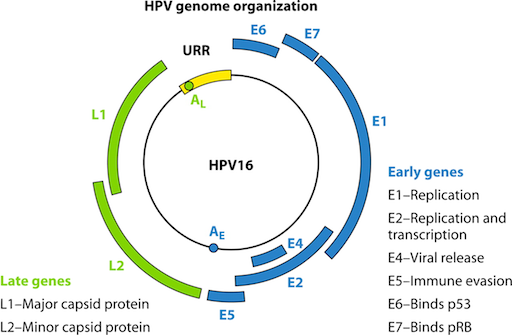
\includegraphics[scale=0.7]{IMG/genoma.png}
	\caption{Cartoon illustrating the genomic organization of a typical mucosal high-risk HPV. The genome contains early and late regions (E), which relate to the positions of the genes within the genome and their timing of expression during the viral life cycle. The early region carries a number of genes which function at the level of viral replication and transcription, i.e., E2, E1, E6, and E7. E2 encodes a protein which has an auxiliary role in viral replication and also functions at the level of transcriptional regulation of the viral early genes. The E6 and E7 genes encode the major transforming proteins of the oncogenic HPVs. The late region (L) encodes viral structural proteins, with L1 being the major capsid protein and L2 being the minor capsid protein.}
	\label{genoma}
\end{figure}
%doi: 10.1128/CMR.05028-11 Clin. Microbiol. Rev. April 2012 vol. 25 no. 2 215-222 1 April 2012

%Foto del HPV-16 con Cryo-EM (nobel química 2017)

The finding was followed by epidemiologists, molecular biologists, vaccinologists, and clinicians culminating in 2006 with the development of effective prophylactic vaccines for human papillomavirus, which have the means to prevent 70-80\% of cervical cancer. Zur Hausen was awarded the Nobel Prize in Physiology or Medicine in 2008, in recognition of his discovery.

\begin{figure}[ht]
	\centering
	
\includegraphics[scale=0.7]{IMG/zurHausen.png}
	\caption{Harald zur Hausen (born 11 March 1936) is a German virologist and professor emeritus. He has done research on cancer of the cervix, where he discovered the role of papilloma viruses, for which he received the Nobel Prize in Physiology or Medicine 2008.}
	\label{zurHausen}
\end{figure} 
%Foto de Zur Hausen

%Datos de lo malo que es
HPV types are often referred to as low risk (LR) wart causing or high risk (HR) cancer causing, based on whether they put a person at risk for cancer.  The types of HPV that can cause genital warts are not the same as the types that can cause cancer.
Persistent human papillomavirus (HPV) infections with genotypes 16 and 18 are responsible for about 70\% of all cervical cancer 
%Clifford GM, Rana RK, Franceschi S, Smith JS, Gough G, Pimenta JM. Human papillomavirus genotype distribution in low-grade cervical lesions: comparison by geographic region and with cervical cancer. Cancer Epidemiol Biomarkers Prev. 2005;14:1157–1164. doi: 10.1158/1055-9965.EPI-04-0812.
%Munoz N, Bosch FX, de Sanjosé S, Herrero R, Castellsague X, Shah KV, et al. Epidemiologic classification of human papillomavirus types associated with cervical cancer. N Engl J Med. 2003;348:518–527. doi: 10.1056/NEJMoa021641.
, with 40-85\% of other anogenital cancers: anal, penile, vaginal, and vulvar cancer, and also 16-28\% of the head and neck cancers.
%%WHO International Agency for Research on Cancer. IARC Monographs on the Evaluation of Carcinogenic Risk to Humans. Human Papillomavirusses. Volume 90. 2007.
%https://www.ncbi.nlm.nih.gov/pmc/articles/PMC4331443/

HPV is a cause of other non malignant diseases, to mention genotypes 6 and 11 cause about 90\% of anogenital warts, and secondarily juvenile onset of recurrent respiratory papillomatosis.
%Lacey CJ, Lowndes CM, Shah KV. Chapter 4: Burden and management of non-cancerous HPV-related conditions: HPV-6/11 disease. Vaccine. 2006;24(Suppl 3):S35–S41. doi: 10.1016/j.vaccine.2006.06.015.

% Literatura dura
Genital human papillomavirus (HPV) is the most common sexually transmitted infection in the United States. More than 40 HPV types can infect the genital areas of men and women, including the skin of the penis, vulva (area outside the vagina), and anus, and the linings of the vagina, cervix, and rectum. These types can also infect the lining of the mouth and throat.

\begin{figure}[ht]
	\centering
	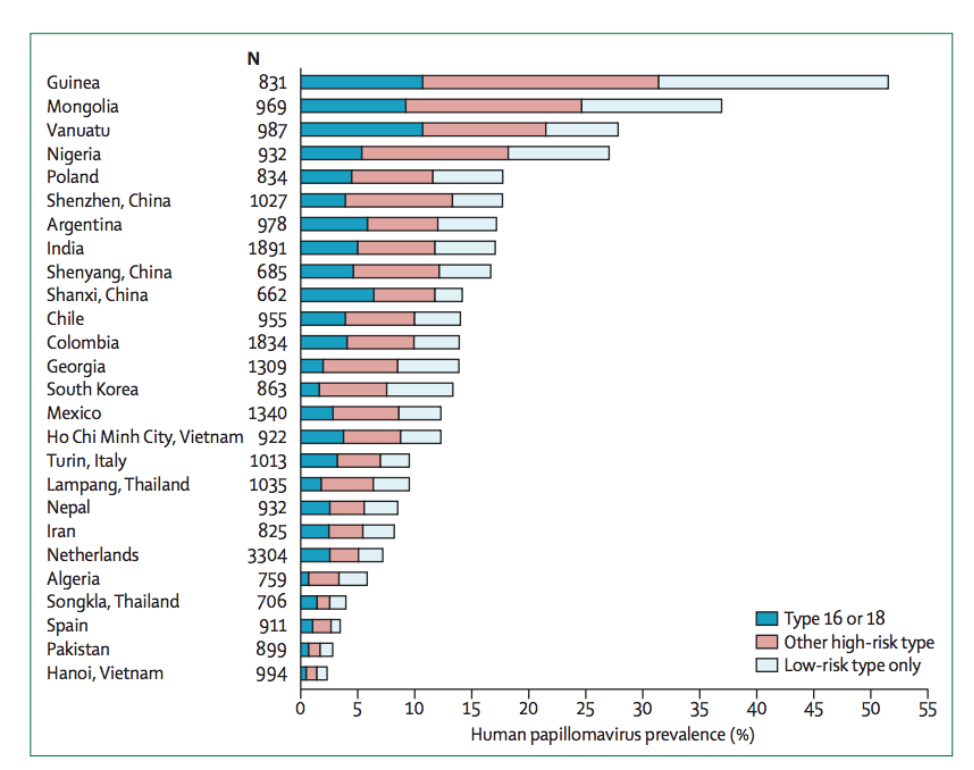
\includegraphics[scale=0.7]{IMG/prevalence.png}
	\caption{Age\-adjusted prevalence of cervical human papillomavirus DNA in sexually active women aged 15\-69 years. Data are from IARC Prevalence Surveys, 1990\-2012.4}
	\label{zurHausen}
\end{figure} 
%Foto de prevalencia


%Literatura
Most people who become infected with HPV do not know they have it. Usually, the body's immune system gets rid of the HPV infection naturally within two years. This is true of both HR and LR types. By age 50, at least 4 out of every 5 women will have been infected with HPV at one point in their lives. HPV is also very common in men, and often has no symptoms.

When the body's immune system can't get rid of a HR HPV infection, it can linger over time and turn normal cells into abnormal cells and then cancer. About 10\% of women with HR HPV on their cervix will develop long-lasting HPV infections that put them at risk for cervical cancer. Similarly, when HR HPV lingers and infects the cells of the vulva, vagina, penis, anus, or the oropharynx (back of the throat, including the base of the tongue and tonsils), it can cause cell changes called precancers. These may eventually develop into cancer if they're not found and removed in time. These cancers are much less common than cervical cancer. Much less is known about how many people with HPV will develop cancer in these areas.

%Empiezo con las vacunas
\section{Vaccines}
Since the release of the first vaccines in 2006, nowadays there are three available: a quadrivalent (including HPV genotypes 16, 18, 6 and 11) and a bivalent vaccine (including genotypes 16 and 18) and a nonavalent (including genotypes 6, 11, 16, 18, 31, 33, 45, 52 and 58). All vaccines are efficacious to protect against precancerous lesions in the cervix, vulva or vagina; in addition, the quadrivalent and nonavalent prevent precancerous anal lesions, anal cancer and anogenital warts.

\begin{figure}[ht]
	\centering
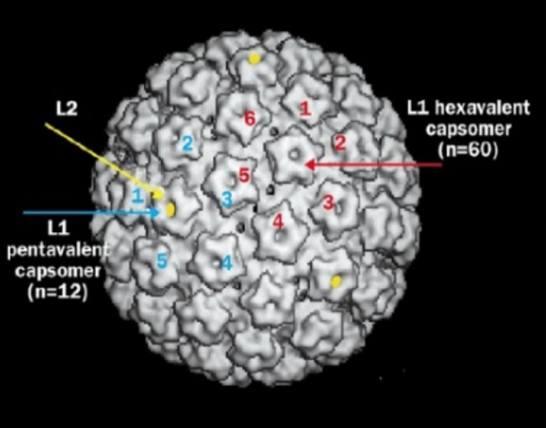
\includegraphics[scale=0.7]{IMG/cryo.png}
\caption{Structure of a HPV virus-like particle. A three-dimensional reconstruction of a cryolectron micrograph (cryo-EM) of a virus-like particle (VLP) is shown. The VLP is composed of 60 hexavalent capsomers and 12 pentavalent capsomers, all consisting of pentamers of L1 protein. The L2 protein is not visible by cryo-EM but is tought to be associated with the pentavalent capsomers, and have been colored in yellow.}
\label{cryo}
\end{figure}  

According to the Advisory Committee on Immunization Practices (ACIP) from the Centers for Disease Control (CDC) and Prevention, new recommendations are given for use of a 2-dose schedule for girls and boys who initiate the vaccination series at ages 9 through 14 years. Three doses remain recommended for persons who initiate the vaccination series at ages 15 through 26 years and for immunocompromised persons.

In Spain HPV vaccine is given to adolescent girls as part of the national immunization programme, and is recommended at different age groups in different Autonomous Communities. Numerous cost-effectiveness studies of HPV-vaccination have been published in other countries. However, few studies include the prophylactic effect of all HPV-associated diseases, or the impact of vaccinating men.

There are countries that recommend also vaccinating boys in order to decrease the burden of disease in them. Some models have shown that the female vaccination program has some herd immunity and the impact of implementing the vaccination in males may not be cost effective, however not vaccinating males leaves them at risk of cancers, especially the groups that do not benefit of the herd immunity, as the males that have sex with males.
Besides, there is no economic analysis of the nonavalent program in Spain, and it is important from the decision making perspective.

Even with the high prevalence of sexually transmitted diseases there are few studies devoted to ascertain the structure of sexual networks and its role in disease transmission. Most studies are restricted to small communities such as the Jefferson High Schools project (P. S. Bearman et al., Chains of Affection: The Structure of Adolescent Romantic and Sexual Networks, American Journal of Sociology, 110(1) (2004) 44-91) or that of Likoma Island (S. Helleringer and H. P. Kohler, Sexual network structure and the spread of HIV in Africa: evidence from Likoma Island, Malawi, AIDS 21 (2007) 2323-2332).

Random network mathematical models may simulate the interactions and propagations of all these viruses through sexual contacts among a population of more than one million people (including heterosexual and homosexual populations). As this model is based upon a network instead of traditional continuous model approaches (E. H. Elbasha et al., Model for assessing human papillomavirus vaccination strategies,  Emerging. Inf. Dis.  2007; 13:28-41) we will be able to determine with higher accuracy the effect of vaccination in a short and large periods of time.

The Human papillomaviruses HPV vaccine induces a herd immunity effect in genital warts when a large number of the population is vaccinated. This aspect should be taken into account when devising new vaccine strategies, like vaccination at older ages or male vaccination. Therefore, it is important to develop mathematical models with good predictive capacities. We devised a sexual contact network that was calibrated to simulate the Spanish epidemiology of different HPV genotypes. Through this model, we simulated the scenario that occurred in Australia in 2007, where 12-13 year-old girls were vaccinated with a three-dose schedule of a vaccine containing genotypes 6 and 11, which protect against genital warts, and also a catch-up program in women up to 26 years of age. Vaccine coverage were $73\%$ in girls with three doses and with coverage rates decreasing with age until $52\%$ for 20-26 year-olds. A fast $59\%$ reduction in the genital warts diagnoses occurred in the model in the first years after the start of the program, similar to what was described in the literature.





\chapter{A first mathematical model of the evolution of the Basque Country population respect to their opinion about ETA under its pressure}\label{paper1}

In this chapter, our objective is to state a first type-epidemiological mathematical model. This model study the evolution over the time of populations in the Basque Country respect their opinions about the ETA's goals. This way, as we mentioned in Section \ref{reduccion}, we want to focus on the evolution of the supporters of ETA's goals to see if they decrease or not.

Here, we recall that popular support is an important enabler for radical violent organizations and it may be crucial for their survival and these extremist groups have also an impact in the societies where they are inserted, especially if those groups are engaged in violent activities. 

The democratic system in the Basque Country and in the rest of Spain is affected by terrorist acts of ETA (murders, kidnapping, vandalism, etc.). Thus, terrorism uses to be one of the most important topics for Spanish public opinion.

In order to carry out this study, the Basque Country' population will be divided into people that:

\begin{itemize}
\item agree with ETA in the objective of independence and the use of
violence to get it,
\item agree with ETA only in the objective of independence, without the use
of violence,
\item completely disagree with ETA.
\end{itemize}

Then, from electoral manifestos and using statistical techniques, in Section \ref{1.1}, a classification of different political parties respect to the political goal "independence" is done. This allows us to divide the Basque population depending on their support to ETA's goals. In Section \ref{1.2} a type-epidemiological mathematical model where the pressure of ETA and its related groups affects the opinion of the people about the support of ETA's goals, is proposed. The model developed in Section \ref{1.2} is not appropriate for data obtained in Section \ref{1.1} (same units), hence Section \ref{1.3} is devoted to scale the model properly to be fitted with classification data obtained in Section \ref{1.4}. Simulations to predict short- and medium-term evolution of population in the Basque Country deterministically and with uncertainty are presented in Section \ref{1.5}. Finally, Section \ref{1.6} is devoted to conclusions.

\section{Classification of ideological groups}\label{1.1}

Let us consider as source data the results of the general elections to the Spanish
Parliament in the Basque Country since June 15th 1977 to March 14th 2004 
\cite{mir}. Since 1977, 85 political parties nominated candidates to,
at least, one general election in the Basque Country electoral district.
General elections data have been considered because, in Spain, experts
consider that general elections give a more realistic political distribution
than local elections \cite{elecGen}.

Now, let us classify the parties with respect to their relation with the
political objective "independence". To do this, a survey is prepared to be
answered from the party's election manifestos. The survey consist of the following
questions (or ideological characteristics):

\begin{enumerate}
\item Nationalist (Yes/No),
\item Religious (Yes/No),
\item Supports violence (Yes/No),
\item Interventionist (Yes/No),
\item Ecologist (Yes/No),
\item Independence (Yes/No),
\item Ideology (right wing or center/left wing/nationalist).
\end{enumerate}

A non-parametric bivariant analysis \cite[Chap. 9]{Groot} is carried out
in order to determine the ideological characteristics (questions of the survey)
related to the use of the violence to get the independence.
These characteristics were "Independence", "Nationalism", "Ideology" and "Support violence"
with associated $p-$values less than $0.01$. In the multiple correspondence
analysis \cite[Chap. 10]{Hair} three different profiles can be seen (see
Figure \ref{1cluster}), nationalist parties agreeing with the independence and
the use of violence, right-wing and center parties against independence
and, in the middle of these profiles, left-wing parties with a non
homogeneous and/or ambiguous position respect to independence and the
use of violence.

\begin{figure}[htb]
\begin{center}
\includegraphics[scale=0.53]{IMG/1cluster.pdf}
\end{center}
\caption{Correspondence analysis shows three different profiles, nationalist 
parties, right-wing and center parties, and left-wing parties with ambiguous 
positions respect to independence and the use of violence.}
\label{1cluster}
\end{figure}

These three profiles (defined by the characteristics "Nationalist", "Independence" "Ideology" and "Support violence") lead us to do a non hierarchical cluster
analysis with three groups of parties, whose definition is determined by the
following characteristics:

\begin{itemize}
\item Group $G_{1}:$ non-nationalist parties against independence and the
use of the violence.
\item Group $G_{2}:$ nationalist parties agreeing with independence but
disagreeing with the use of the violence.
\item Group $G_{3}:$ nationalist parties agreeing with independence and the use
of the violence.
\end{itemize}

The above division of political parties allows us to classify the population depending on the parties they vote and the position of these parties respect to ETA's goals. With this approach, the population of the Basque Country can be divided into four subpopulations

\begin{itemize}
\item $E(t)$, number of people who share the common ideological
characteristics of parties in $G_{1}$ at time $t,$
\item $N(t)$, number of people who share the common ideological
characteristics of parties in $G_{2}$ at time $t,$
\item $V(t)$, number of people who share the common ideological
characteristics of parties in $G_{3}$ at time $t,$ and
\item $A(t)$, the rest of the people at time $t$. It includes
people who do not share the ideological characteristics of groups $G_{1},$ 
$G_{2}$ and $G_{3}$ or people who abstain.
\end{itemize}

Figure \ref{1graf1} shows the percentage of votes of each subpopulation in
each election. 

\begin{figure}[htb]
\begin{center}
\includegraphics[scale=0.62]{IMG/1datos.pdf}
\end{center}
\caption{This figure shows the percentage of votes of each subpopulation 
in each election. Vertical lines correspond to electoral days. Let us 
consider in our study data between $1979$ and $1996$, where most of the  
time the Socialist Party (PSOE) was in the government, and the same policy against terrorism can 
be assumed.}
\label{1graf1}
\end{figure}

Two considerations should be mentioned here to understand some trend changes in
Figure \ref{1graf1} at the beginning and at the end. The general elections in
1977 were the first celebrated after the dictator Franco died. Lots of
parties presented candidates, the political situation was not clear and it
is reflected in the data. In 2000, political parties in group $G_{3}$ asked abstention and in $2004$, the "Law of Political Parties" (LPP) forbade these parties from nominating candidates. In fact, LPP outlawed the political parties that did not condemn the violence. Notice that in $2000$ and $2004$ abstention increased, but this was because the votes for parties of group $G_{3}$ were considered void, increasing the subpopulation $A\left( t\right)$.

All the above leads us to consider only election data since 1979 to 1996
where the major part of time the Socialist Party (PSOE) governed Spain and
the same policy against terrorism can be assumed in order to fit the
model we will develop in Section \ref{1.2}.

\begin{table}[htb]
\label{1Table1}
\begin{center}
\begin{tabular}{ccccc}
\hline
Election date & $E(t)$ & $N(t)$ & $V(t)$ & $A(t)$ \\ \hline
\multicolumn{1}{l}{Jun 15th, 1977} & \multicolumn{1}{l}{$0.435392$} & 
\multicolumn{1}{l}{$0.266825$} & \multicolumn{1}{l}{$0.0316636$} & 
\multicolumn{1}{l}{$0.26612$} \\ 
\multicolumn{1}{l}{Mar 1st, 1979} & \multicolumn{1}{l}{$0.278466$} & 
\multicolumn{1}{l}{$0.233303$} & \multicolumn{1}{l}{$0.0967287$} & 
\multicolumn{1}{l}{$0.391502$} \\ 
\multicolumn{1}{l}{Oct 28th, 1982} & \multicolumn{1}{l}{$0.347978$} & 
\multicolumn{1}{l}{$0.306366$} & \multicolumn{1}{l}{$0.114331$} & 
\multicolumn{1}{l}{$0.231325$} \\ 
\multicolumn{1}{l}{Jun 22nd, 1986} & \multicolumn{1}{l}{$0.294959$} & 
\multicolumn{1}{l}{$0.245271$} & \multicolumn{1}{l}{$0.117587$} & 
\multicolumn{1}{l}{$0.342183$} \\ 
\multicolumn{1}{l}{Dec 17th, 1989} & \multicolumn{1}{l}{$0.246631$} & 
\multicolumn{1}{l}{$0.283516$} & \multicolumn{1}{l}{$0.111871$} & 
\multicolumn{1}{l}{$0.357982$} \\ 
\multicolumn{1}{l}{Jun 6th, 1993} & \multicolumn{1}{l}{$0.330461$} & 
\multicolumn{1}{l}{$0.234575$} & \multicolumn{1}{l}{$0.100969$} & 
\multicolumn{1}{l}{$0.333994$} \\ 
\multicolumn{1}{l}{Mar 3rd, 1996} & \multicolumn{1}{l}{$0.364871$} & 
\multicolumn{1}{l}{$0.236203$} & \multicolumn{1}{l}{$0.0872077$} & 
\multicolumn{1}{l}{$0.311718$} \\ 
\multicolumn{1}{l}{Mar 12th, 2000} & \multicolumn{1}{l}{$0.364974$} & 
\multicolumn{1}{l}{$0.239676$} & \multicolumn{1}{l}{$0.$} & 
\multicolumn{1}{l}{$0.39535$} \\ 
\multicolumn{1}{l}{Mar 14th, 2004} & \multicolumn{1}{l}{$0.382756$} & 
\multicolumn{1}{l}{$0.299592$} & \multicolumn{1}{l}{$0.$} & 
\multicolumn{1}{l}{$0.317652$} \\ \hline
\end{tabular}
\end{center}
\caption{Data corresponding to graphic in Figure \ref{1graf1}.}
\end{table}

Taking into account that, in Spain, only people older than $18$ can vote and
supposing that children and teenagers have the same way of thinking as their
parents, let us assume that data in Table \ref{1Table1} gives a general voting distribution 
of the whole population in the Basque Country, and taking into account the classification of parties, 
the distribution of the people depending on their support to ETA's goals.

\section{Building the type-epidemiological mathematical model}\label{1.2}

Let us consider the population of the Basque Country divided into four
subpopulations determined in Section \ref{1.1}, that is, $E,$ $N,$ 
$V$ and $A$. Also, we assume that:

\begin{itemize}
\item The number of births $\Lambda(t)$ and the number of
deaths $\Phi(t)$ in the year $t$, are proportional to the number of individuals
in each subpopulation.

\item Terrorism does not increase substantially the number of deaths. 

\item The immigration $\Gamma(t)$ and emigration $\Sigma(t)$ in Basque Country 
are also included. It is considered that immigration and emigration only occurs 
in subpopulations $E$ and $A$ due to the terror pressure \cite{exilio2, exilio3, exilio1} 
in proportions $\alpha_{1}$ and $\alpha_{2}$, respectively, to be determined.
\end{itemize}

In order to determine the rest of transition terms, 
partial correlation coefficients have been used. This coefficient studies
the linear relation between two variables under the influence of a third
variable \cite{Groot}. To carry out this study, let us take data of Table
\ref{1Table1} corresponding to elections from March 1st 1979 to March 3rd
1996.

The partial correlation coefficient between subpopulations $E$ and $A$ under
the influence of $V$ is $-0.8409$ with a $p-$value of $0.009$ ($p-value < 0.05$). It means that
there is a linear inverse relation between $E$ and $A$ under $V,$ that is,
under $V$ an increasing of subpopulation $E$ implies a decrease of
subpopulation $A$ and vice versa. Moreover, the linear correlation
coefficient between $E$ and $A$ without the presence of $V$ is not
significant. Therefore the transition between $E$ and $A$ is not linear because it is only possible under the influence of population $V$, and it is modeled by the nonlinear term

\[
\beta_{1} E(t) \frac{V(t)}{T(t)}, 
\]

where $\beta_{1} > 0$ indicates that the transition is due to the pressure of
violent acts and $\beta_{1} < 0$ indicates a law enforcement.

Analogously, a similar situation occurs between subpopulations $A$ and $V$
under the pressure of $V$. Then, the transition between subpopulations $A$
and $V$ is modeled by the nonlinear term

\[
k \beta_{1} A(t) \frac{V(t)}{T(t)}, 
\]

with $k > 0$.

On the other hand, the partial correlation coefficient between
subpopulations $N$ and $A$ under the influence of $E$ is $-0.6292$ with a 
$p- $value of $0.05$ and there is a linear inverse relation between $N$ and 
$A $ under $E$. Also, the linear correlation coefficient between $N$ and $A$
without the presence of $E$ is not significant. Therefore the transition
between $N$ and $A$ is modeled by the nonlinear term

\[
\beta_{2} N(t) \frac{E(t)}{T(t)}. 
\]

Then, the system of differential equations that models the evolution over the time of populations in the Basque Country respect their opinions about the ETA's goals under the pressure of its violence is given by

\begin{eqnarray}
E'(t)	& = &	\Lambda(t) E(t) + \alpha_{2} \Gamma(t) - \beta_{1} E(t) \frac{V(t)}{T(t)} - \label{1m1} \\
        &   &	\Phi(t) E(t) - \alpha_{1} \Sigma(t),  \nonumber \\                          
N'(t)	& = &	\Lambda(t) N(t) - \beta_{2} N(t) \frac{E(t)}{T(t)} - \Phi(t) N(t),  \label{1m2} \\
V'(t)	& = &	\Lambda(t) V(t) + k \beta_{1} A(t) \frac{V(t)}{T(t)} - \Phi(t) V(t),  \label{1m3} \\
A'(t)	& = &  	\Lambda(t) A(t) + (1 - \alpha_{2}) \Gamma(t) + \beta_{1} E(t) \frac{V(t)}{T(t)} + \label{1m4} \\
		&   &	\beta_{2}N(t) \frac{E(t)}{T(t)} - k \beta_{1} A(t) \frac{V(t)}{T(t)} - \Phi(t) A(t) - 
		        (1 - \alpha_{1}) \Sigma(t),  \nonumber \\
T(t)		& = &	E(t) + N(t) + V(t) + A(t).  \label{1m5}
\end{eqnarray}

The above system of differential equations can be represented by the diagram of Figure \ref{1diagrama}.

\begin{figure}[htb]
\begin{center}
\includegraphics[scale=0.48]{IMG/1DiagramaModeloFanatismo.pdf}
\end{center}
\caption{Diagram corresponding to the model defined by the system of 
differential equations $\left( \protect\ref{1m1}\right) -\left( \protect\ref{1m5}\right).$}
\label{1diagrama}
\end{figure}

\section{Scaling the model $(\ref{1m1}) -(\ref{1m5})$}\label{1.3}

Data obtained in Section \ref{1.1} is related to the percentages of
population while model $\left( \ref{1m1}\right) -\left( \ref{1m5}\right)$
is related to the number of individuals. It leads us to transform (by scaling) the
model into the same units as data, because one of our objectives is to fit the
data with the model in next section.

Hence, following ideas developed in \cite{Martcheva, Mena, scaling} about how
to scale models where the population is varying in size, adding equations 
$\left( \ref{1m1}\right) -\left( \ref{1m4}\right)$ it is obtained

\begin{equation}
T^{\prime }\left( t\right) =\left[ \Lambda \left( t\right) -\Phi \left(
t\right) \right] T\left( t\right) +\Gamma \left( t\right) -\Sigma \left(
t\right).  \label{1eqT}
\end{equation}

Dividing both members of $\left( \ref{1eqT}\right) $ by $T\left( t\right) $
we have that

\begin{equation}
\frac{T^{\prime }\left( t\right) }{T\left( t\right) }=\Lambda \left(
t\right) -\Phi \left( t\right) +\frac{\Gamma \left( t\right) -\Sigma \left(
t\right) }{T\left( t\right) }.  \label{1T/T}
\end{equation}

On the one hand, if we define the rates (depending on time)

\begin{equation}
e=\frac{E}{T},n=\frac{N}{T},v=\frac{V}{T},a=\frac{A}{T},\gamma =\frac{\Gamma 
}{T},\sigma =\frac{\Sigma }{T},  \label{1ratios}
\end{equation}

equation $\left( \ref{1T/T}\right) $ can be transformed into

\begin{equation}
\frac{T^{\prime }}{T}=\Lambda -\Phi +\gamma -\sigma .  \label{1T/Tcorta}
\end{equation}

On the other hand, let us compute the derivative of $e,$ defined in 
$\left(\ref{1ratios}\right).$ Using $\left(\ref{1T/Tcorta}\right)$ we obtain that,

\begin{equation}
e^{\prime }=\frac{E^{\prime }T-ET^{\prime }}{T^{2}}=\frac{E^{\prime }}{T}-
\frac{E}{T}\frac{T^{\prime }}{T}=\frac{E^{\prime }}{T}-e\left[ \Lambda -\Phi
+\gamma -\sigma \right] .  \label{1chulla}
\end{equation}

In an analogous way, we also have that,

\begin{eqnarray*}
n^{\prime } &=&\frac{N^{\prime }}{T}-n\left[ \Lambda -\Phi +\gamma -\sigma 
\right] , \\
v^{\prime } &=&\frac{V^{\prime }}{T}-v\left[ \Lambda -\Phi +\gamma -\sigma 
\right] , \\
a^{\prime } &=&\frac{A^{\prime }}{T}-a\left[ \Lambda -\Phi +\gamma -\sigma 
\right] .
\end{eqnarray*}

Now, consider equation $\left( \ref{1m1}\right) .$ If we divide it by $T,$ we
have

\[
\frac{E^{\prime }}{T}=\Lambda \frac{E}{T}+\alpha _{2}\frac{\Gamma }{T}-\beta
_{1}\frac{E}{T}\frac{V}{T}-\Phi \frac{E}{T}-\alpha _{1}\frac{\Sigma }{T}, 
\]

using $\left( \ref{1chulla}\right) $ and substituting by the corresponding
rates defined in $\left( \ref{1ratios}\right) $ one gets 

\[
e^{\prime }+e\left[ \Lambda -\Phi +\gamma -\sigma \right] =\Lambda e+\alpha
_{2}\gamma -\beta _{1}ev-\Phi e-\alpha _{1}\sigma , 
\]

obtaining the scaled equation

\begin{equation}
e^{\prime }=\left( \sigma -\gamma \right) e+\alpha _{2}\gamma -\beta
_{1}ev-\alpha _{1}\sigma .  \label{1sm1}
\end{equation}

The remaining equations can be scaled in the same way to obtain

\begin{eqnarray}
n^{\prime } &=&\left( \sigma -\gamma \right) n-\beta _{2}ne,  \label{1sm2} \\
v^{\prime } &=&\left( \sigma -\gamma \right) v+k\beta _{1}av,  \label{1sm3} \\
a^{\prime } &=&\left( \sigma -\gamma \right) a+\left( 1-\alpha _{2}\right)\gamma +\beta _{1}ev+ \label{1sm4} \\
            & &\beta _{2}ne-k\beta _{1}av-\left( 1-\alpha _{1}\right) \sigma. \nonumber 
\end{eqnarray}

Notice that the scaled system of differential equations $\left( \ref{1sm1}
\right) -\left( \ref{1sm4}\right) $ is also a non-autonomous system because
the immigration $\left( \gamma \right) $ and emigration $\left( \sigma
\right) $ rates depend on time.

\section{Model fitting}\label{1.4}

Taking data in Table \ref{1Table1} corresponding to elections from March 1st
1979 to March 3rd 1996, let us to fit data with the scaled model 
$\left( \ref{1sm1}\right) -\left( \ref{1sm4}\right).$

Moreover demographic data from \cite{demogPV}, in particular annual
population, immigration and emigration data in the interval 1979 to 1996 are
considered. Hence, in order to compute immigration and emigration rate
functions $\gamma \left( t\right) $ and $\sigma \left( t\right),$ we divide
each immigration and emigration datum by the corresponding population datum.
Then, we use piecewise linear interpolation to construct both functions, $\gamma$ and 
$\sigma $. Migration data are depicted in Figure \ref{1migra}.

\begin{figure}[htb]
\begin{center}
\includegraphics[scale=0.8]{IMG/1migracion.pdf}
\end{center}
\caption{Immigration and emigration rates from 1979 until 2015. Notice that from 2005 these rates are constant, equal to the ones in 2005.}
\label{1migra}
\end{figure} 

As initial condition of the model $\left( \ref{1sm1}\right) -\left(\ref{1sm4}\right),$ 
it is considered

\begin{equation}
\begin{array}{cc}
E\left( t_{0}\right) =0.278466, & N\left( t_{0}\right) =0.233303, \\ 
V\left( t_{0}\right) =0.0967287, & A\left( t_{0}\right) =0.391502,
\end{array}
\label{1IC}
\end{equation}

where $t_{0}$ corresponds to March 1st 1979 (see Table \ref{1Table1}). In
order to compute the best fitting, we carried out computations with 
\emph{Mathematica} \cite{Wolfram} and we implemented the function

\[
\begin{array}{ccccc}
\mathbb{F} & : & \mathbb{R}^{5} & \longrightarrow & \mathbb{R} \\ 
&  & \left( \beta _{1},\beta _{2},k,\alpha _{1},\alpha _{2}\right) & 
\longrightarrow & \mathbb{F}\left( \beta _{1},\beta _{2},k,\alpha
_{1},\alpha _{2}\right)
\end{array}
\]

which variables are $\beta _{1},$ $\beta _{2},$ $k,$ $\alpha _{1}$ and 
$\alpha _{2}$ such that:

\begin{enumerate}
\item Solve numerically (using \textit{Mathematica} command \emph{NDSolve[]}) the system of differential
equations $\left( \ref{1sm1}\right) -\left( \ref{1sm4}\right) $ with initial
values $\left( \ref{1IC}\right),$

\item For $t=$ Oct 28th 1982, Jun 22nd 1986, Dec 17th 1989, Jun 6th 1993 and
Mar 3rd 1996, corresponding to election days, evaluate the computed
numerical solution for each subpopulation $E\left( t\right) ,$ $N\left(
t\right) ,$ $V\left( t\right) ,$ $A\left( t\right) $.

\item Compute the mean square error between the values obtained in Step 2
and the electoral data from Oct 28th 1982 to Mar 3rd 1996, (Table 
\ref{1Table1}).
\end{enumerate}

Function $\mathbb{F}$ takes values in $\mathbb{R}^{5}$ ($\beta _{1},$ 
$\beta_{2},$ $k,$ $\alpha _{1}$ and $\alpha _{2})$ and returns a positive real
number. Hence, we minimize this function using the Nelder-Mead
algorithm \cite{Nelder, Press}, that does not need the computation of
any derivative or gradient, which is impossible to know in this case. Thus, the values of $\beta _{1},$ $\beta _{2},$ $k,$ 
$\alpha _{1}$ and $\alpha _{2},$ with restrictions $0\leq \alpha _{1},\alpha_{2}\leq 1$ and $k>0,$ that minimize the function $\mathbb{F}$ are

\begin{equation}
\begin{array}{l}
\beta_{1}=0.0534,\ \beta_{2}=-0.0338,\\
 k=0.5352,\\
\alpha_{1}=0.8945,\ \alpha_{2}=0.9999.  
\end{array}
\label{1parametros}
\end{equation}

Parameters indicate that population flows from $E$ to $A$ and from $A$ to $V$ ($\beta_{1}, k > 0$), and from $A$ to $N$ ($\beta_{2} < 0$) very slowly. Furthermore, the value of $k$ indicates that the pressure of $V$ affects twice to $E$ than to $A$. Additionally, almost all emigration and immigration occurs in subpopulation $E$ ($\alpha_{1}=0.8945$, $\alpha_{2}=0.9999$). 

\section{Trends over next few years}\label{1.5}

Once the model parameters have been estimated, under the assumption that government anti-terrorist policies and ETA strategies do not change, we can use the model to predict the trend of each subpopulation until $2020$, i.e., the deterministic prediction. To do so, demographic data from \cite{demogPV} are used: immigration and emigration available data go from 1977 until 2008 and the 2008 datum is repeated until 2020; real population data from 1975 to 2008 are available and also predictions until 2020. 

Then, we use the model parameters obtained in (\ref{1parametros}), substitute them into the model and obtain the model forecasting for next electoral years $2012$, $2016$ and $2020$. The results can be seen in Table \ref{1Table2}.

\begin{table}[ht]
\begin{center}
\begin{tabular}{c|cccc}
  &  $E$ & $N$ & $V$ & $A$ \\
 \hline    
\begin{tabular}{l}
 $2012$ \\  $2016$\\  $2020$
\end{tabular}
&  
\begin{tabular}{c}
  0.343714 \\ 0.359023 \\ 0.373446
\end{tabular}
 & 
\begin{tabular}{c}
  0.291674\\	0.296761	\\ 0.302587
\end{tabular}
 & 
\begin{tabular}{c}
  0.114067 \\ 0.113756 \\	0.113205
\end{tabular}
& 
\begin{tabular}{c}
  0.250546\\	0.23046\\0.210763
\end{tabular}
\end{tabular}
\end{center}
\caption{Deterministic prediction for the next electoral years $2012$, $2016$ and $2020$. } 
\label{1Table2}
\end{table}

Looking at Tables \ref{1Table1} (data from $1979$ to $1996$) and \ref{1Table2} jointly, we can observe a slight increase in groups $E$, $N$ and $V$ at the expense of $A$. It is noteworthy to see how subpopulation $V$ has hardly varied during the 40 years studied. 

However, as we mentioned in the Introduction chapter, uncertainty is a key part dealing with Social Sciences phenomena. Therefore, the supposition that parameters always remain constant or data in Table \ref{1Table1} and demographic data do not contain errors, is not appropriate. Thus, it is natural to consider that the model parameters $\beta_{1}$, $\beta_{2}$, $k$, $\alpha_{1}$ and $\alpha_{2}$ contain uncertainties. Hence, the deterministic prediction can give us an idea about future trends but, in this case, the obtained values may not be accurate.

Therefore, we propose forecasting future trends using confidence intervals. In order to calculate these confidence intervals, let us use the technique called Latin Hypercube Sampling (LHS) to vary parameter values in the proposed model. LHS, a type of stratified Monte Carlo sampling, is a sophisticated and efficient method for achieving equitable sampling of all input parameters simultaneously \cite{BLOWER, OLSSON}. Each parameter for a model can be defined as having an appropriate probability density function associated with it. It is usual to use the uniform distribution centred at deterministic parameter estimators in absence of data to give information as to the distribution for a given parameter \cite{MCKAY, OLSSON}. Thus, the model can be simulated by sampling a single value from each parameter distribution. Many samples should be taken and many simulations should be run, producing variable output values that can be treated with descriptive statistic techniques to compute the means and $90\%$ confidence intervals.

An important issue arises here and it is how much we should vary the parameters to quantify uncertainty. Some studies analyse the effect on populations of health campaigns \cite{SNYDER}, electoral campaigns \cite{FOURNIER} or the bombing attacks in Madrid few days before elections \cite{BALI}, and all of them over a short period. In these cases, what we call "effect" refers to a change of opinion to adopt a healthier way of life, to leave the abstention group and vote or to switch party. This change of opinion is about $5\%$ in health campaigns \cite{SNYDER}, $5\%-19\%$ in Canadian electoral campaigns depending on the time of decision \cite{FOURNIER} and around $10\%$ in the elections immediately after attacks in Madrid \cite{BALI}. Moreover, the referred changes are related to population, not to parameters and therefore, not related to rates of political ideology change. However, as we mentioned before, anti- or pro-terrorist policies and strategies are designed to change the value of the model parameters. Thus, even though we do not have any quantification of uncertainty in the parameters, let us assume that they may have a variation not greater than $20\%$ of their values, i.e., 

\begin{equation}
	\begin{array}{c}
		\beta_{1} \in [0.0428, 0.0642],\ \beta_{2} \in [-0.0270, -0.0406], \\ 
		\alpha_{1} \in [0.7156, 1],\ \alpha_{2} \in [0.78, 1].
	\end{array}
	\label{1int}
\end{equation}

Note that $20\%$ variation of $\beta_{1}$ implies $20\%$ variation of $k \beta_{1}$. Now, applying the LHS technique with $5,000$ samples using uniform distributions centred at the deterministic parameter values (\ref{1parametros}), i.e., for $5,000$ different $5-$tuples $(\beta_{1}, \beta_{2}, k, \alpha_{1}, \alpha_{2}),$ we solve the model to obtain $5,000$ outputs 

$$(E(t_f), N(t_f), V(t_f), A(t_f)),$$ 

for $t_f= 2012, 2016, 2020$, the coming electoral years. Hence, for each $t_f$ and for each subpopulation we can compute the $90\%$ confidence interval from the corresponding $5,000$ outputs. Results can be seen in Table \ref{1Table3}.

\begin{table}[ht]
\begin{center}
\begin{tabular}{c|cccc}
  &  $E$ & $N$ & $V$ & $A$ \\
 \hline
 $2012$	& $[0.261,0.37]$ & $[0.267,0.307]$ & $[0.109,0.124]$	 & $[0.217,0.345]$ \\
 $2016$	& $[0.266,0.387]$ & $[0.268,0.315]$ & $[0.108,0.125]$	 & $[0.196,0.337]$ \\
 $2020$	& $[0.271,0.404]$ & $[0.27,0.324]$ & $[0.107,0.126]$	 & $[0.173,0.33]$ 
\end{tabular}
\end{center}
\caption{$90\%$ confidence intervals obtained with $5,000$ model outputs using LHS technique in the next electoral years $2012$, $2016$ and $2020$. } 
\label{1Table3}
\end{table}

The results obtained in the present section are summarised in Figure \ref{1ajuste}. The parts of each graph are: 

\begin{itemize}
\item the points on the left are data from Table \ref{1Table1}; 
\item the continuous line is the deterministic model output for parameters in (\ref{1parametros}); 
\item the $90\%$ confidence intervals in $2012$, $2016$ and $2020$ are on the right; 
\item the points in the middle of the confidence intervals are the mean of $5,000$ outputs for each subpopulation and each electoral year.
\end{itemize}

\begin{figure}[htb]
\includegraphics[scale=0.8]{IMG/1AjustePrediccionCI.pdf}
\caption{Model fitting since March 1st 1979 to March 3rd 1996 and future prediction for each subpopulation, $E,$ $N,$ $V$ and $A.$ Points on the left are data of election days, the continuous lines the solution of the model until 2020. The $90\%$ confidence intervals for electoral years with their mean are on the right.}
\label{1ajuste}
\end{figure}

Figure \ref{1ajuste} allows us to say, on the one hand, that $E$ and $A$ are the ideological groups with more uncertainty, $10.9\%-13.3\%$ and  $12.5\%-15.6\%$ respectively (maximum and minimum length of their respective confidence intervals in Table \ref{1Table3}), where the deterministic prediction is far from the mean of the confidence intervals. This brings up some doubts as to the deterministic prediction, to consider more conservative predictions than the one obtained with LHS one and to point out the high sensitivity of groups $E$ and $A$ to model parameter perturbations (policy changes). On the other hand, subpopulations $N$ and $V$ have few uncertainty, $4\%-5.4\%$ and $1.5\%-1.9\%$ respectively, and the deterministic prediction is very close to the mean of confidence intervals. This leads us to say that there is a minor flow across groups $V$ and $N$. Even though the confidence interval variations are greater than the ones in $V$, the population in $N$ is almost three times the one in $V$ and the variation $4\%-5.4\%$ of $N$ is less than three times the one of $V$. It also suggests that subpopulations $N$ and $V$ are less sensitive to model parameter perturbations (policy changes).

\section{Conclusions}\label{1.6}

In this chapter, we propose a type-epidemiological model to analyse the evolution over the time of populations in the Basque Country respect their opinions about the ETA's goals, taking into account that ETA uses violence to demand Basque independence from Spain. 

Using this model and applying the Latin Hypercube Sampling, we predict ideological trends over the next few years giving $90\%$ confidence intervals. The application of LHS is our first approach in dealing with model uncertainty, but in this case with an important drawback as is the quantification of the variation of the model parameters and the probability distribution they follow. We will attempt to overcome these inconveniences in the following chapters.

\textbf{Remark.} As we mentioned in the Introduction chapter, a paper including some results presented in this chapter was rejected to be published. One of the main drawbacks mentioned was related to the division into subpopulations, because the division was not well done and as a consequence, the predictions given in Table \ref{1Table3} are far to be correct. For instance, we predict a result of $10.9\% - 12.4\%$ for parties in $V$ for elections in year 2012 and, as we said in Chapter \ref{ETA} the parties included in $V$ obtained around $25\%$ of votes, being the second most voted parties in the Basque Country. Moreover, an electoral prediction over the next three election dates ($12$ years) may be considered too long. 

Therefore, although the model presented here was well considered by some referees and colleagues, it is only a rough approach to the problem. This is an example of the difficulty of modelling in Social Sciences.

However, we contacted with an expert who addressed our work and this is reflected in the following chapters.

%\chapter{The effect of the Spanish \textit{Law of Political Parties} (LPP) on the attitude of the Basque Country population towards ETA}\label{paper2}

In Chapter \ref{paper1} we presented a first approach and detected several drawbacks. With the help of the expert we focus and improve the model. Also, we use other techniques to deal with the model uncertainty in order to avoid the detected inconveniences.

As we described in Chapter \ref{ETA}, in Jun 2002, the Spanish Government passed the "Law of Political Parties" (LPP) with the aim, among others, to prevent parties giving political support to terrorist organizations. This law affected the Basque nationalist party Batasuna, due to its proved relation with ETA. 

Along with that impact in the political arena, it is also reasonable to expect some impact in the sociological one. The question is: did the LPP have any effect on the attitude of the Basque Country population towards ETA? This question is particularly pertinent in light of the current situation in that region. On the one hand, generally speaking, it is well known that repressive initiatives taken by governments can generate sympathies, to some degree, towards the repressed organizations. On the other hand, in this particular case, violent activities carried out by ETA could be responsible for part of the population not expressing their political beliefs freely, so measures taken to prevent ETA's violence could encourage people to express themselves more openly. In other words, either has ETA together with its political wings, gained additional support from the population or has part of the Basque country been uninhibited because of that law? 

In order to study this problem, we use a new data set from the Euskobarometro survey \cite[Table 20]{eusko}, one of the best-known independent opinion polls in the region, which is periodically conducted by the University of the Basque Country. The period of time considered for this study is from the passing of the LPP (Jun 2002) to May 2005. The reason for this time limitation is that, in our opinion, during this period the anti-terrorist policies were reasonably homogeneous, while, from May 2005 on, a perceptible change occurred when the Congress approved the possibility the Government supports a dialogue process with ETA given that appropriate conditions to end violence occur \cite[Resoluci\'on 34, p. 13]{Congreso}. It is believed that this major event, and subsequent ones as well, could jeopardize the homogeneity necessary to conduct this study\footnote{A month later, ETA announced the cessation of its armed actions against the elected politicians in Spain, although later on it pointed out that this truce did not apply to members of the Government.}. Finally, remark that during the mentioned period of time, the 11-M bombing attacks in Madrid (on 11 March 2004), did not provoke major changes in the trend. We justified this in Chapter \ref{ETA}.

This chapter is organized as follows. In Section \ref{2.1}, data from Euskobarometro about the attitude of the Basque Country population towards ETA are retrieved and processed \cite[Table 20]{eusko}. Section \ref{2.2} is devoted to building a model describing the attitude dynamics towards ETA in the Basque Country. Model parameters are estimated in Section \ref{2.3} by fitting the model with the Euskobarometro data. In Section \ref{2.4} it is concluded that the LPP is responsible for an increasing attitude of rejection towards ETA and we quantify this effect by using a bootstrapping approach. Finally, some conclusions are drawn in Section \ref{2.5}.

\section{Data}\label{2.1}
In this case we are not going to use electoral data. Instead, we use data series from Euskobarometro. This was suggested by the expert because Euskobarometro appears every six months (is more regular) and it asks for a lot of relevant sociological and political questions in the Basque Country. Furthermore, when an individual vote to a political party, he/she does not necessarily assume and support all the ideas of the political party.
 
Thus, we have retrieved data series from the Euskobarometro of Nov 2010 on the attitude of the Basque Country population towards ETA \cite[Table 20]{eusko}. The eight types of attitudes towards ETA that appear in the Euskobarometro are as follows: Total support; Justification with criticism; Goals yes / Means no; Before yes / Not now; Indifferent; ETA scares; Total rejection; No answer. In order to simplify the model (the number of subpopulations) we group the eight attitudes in only three.

\begin{enumerate}
\item Support: people who have an attitude of support towards ETA. We consider the people with attitudes of "Total support" and "Justification with criticism" make up of this group.
\item Rejection: people who have an attitude of rejection against ETA. In this group we include the people with attitudes "Goals yes / Means no", "Before yes / Not now", "ETA scares" and "Total rejection". It could be questionable to include in this group the attitude "Goals yes / Means no", however, the fact is that there are parties and associations in the Basque Country with similar goals as ETA  and they have a rejection attitude towards ETA because of its violent means. 
\item Abstention: people who have no opinion or have an indifferent attitude towards ETA, that is, the "Indifferent" and the "No answer" groups.
\end{enumerate}

Data grouped in these three groups appear in Table \ref{2TABLA2} from May 1995 to May 2002 (before the passing of the LPP) and Table \ref{2TABLA3} for the period from Nov 2002 to May 2005 (after the passing of the LPP until the granting of permission by the Spanish Parliament to conduct a dialogue with ETA).

\begin{table}[ht]
\centering
\begin{tabular}{|l|c|c|c|}
\hline
  Survey date  & Support (\%) & Rejection (\%) & Abstention (\%) \\ 
\hline
 May 1995 & 7	&85	&8 \\
 Nov 1995 & 5	&87	&8 \\
 Nov 1996 & 6	&87	&7 \\
 Nov 1997 & 6	&86	&8 \\
 Nov 1998 & 5	&85	&10 \\
 May 1999 & 11	&76	&13 \\
 May 2000 & 8	&87	&5 \\
 Nov 2000 & 7	&87	&6 \\
 May 2001 & 3	&90	&7 \\
 Nov 2001 & 4	&88	&8 \\
 May 2002 & 2	&96	&2 \\
 \hline 
\end{tabular} 
\caption{Percentage of people in the Basque Country with respect to their attitude towards ETA from May 1995 to May 2002, when  the LPP was passed (pre-LPP scenario).}
\label{2TABLA2} 
\end{table}

\begin{table}[ht]
\centering
\begin{tabular}{|l|c|c|c|}
\hline
     Survey date  & Support (\%) & Rejection (\%) & Abstention (\%) \\ 
\hline
 Nov 2002 & 3	&	93	&	4 \\
 May 2003 & 2 &	95	&	3 \\
 Nov 2003 & 2	&	94	&	4 \\
 May 2004 & 3	&	93	&	4 \\
 Nov 2004 & 3	&	93	&	4 \\
 May 2005 & 2 &	93	&	5 \\
 \hline 
\end{tabular} 
\caption{Percentage of people in the Basque Country with respect to their attitude towards ETA from Nov 2002 to May 2005, after the passing of the LPP until the granting of the permission by the Spanish Parliament to conduct a dialogue with ETA (post-LPP scenario).}
\label{2TABLA3} 
\end{table}

The data in Table \ref{2TABLA2} will help us to estimate the parameters of the mathematical model. The data in Table \ref{2TABLA3} will be used to find out if the LPP affected the attitude of the people in the Basque Country towards ETA, and if so, quantify the effect of the LPP.

\section{Model building}\label{2.2}  
Bearing in mind Tables \ref{2TABLA2} and \ref{2TABLA3}, we distinguish three main different attitudes towards ETA and divide the population of the Basque Country into the following three subpopulations (time $t$ in years):

\begin{itemize}
\item $A_1(t)$, the percentage of people in the Basque Country who have an attitude of support towards ETA at time instant $t$,
\item $A_2(t)$ is the percentage of people who have an attitude of rejection towards ETA at time $t$, 
\item $A_3(t)$ corresponds to the percentage of population in the Basque Country whose attitude towards ETA is not defined, who abstain, or who simply do not want to state their opinion, at time $t$.
\end{itemize}

$A_1(t)$, $A_2(t)$ and $A_3(t)$ are the variables of the mathematical model. The assumptions used to build the equations of the model are as follows.

\begin{itemize}
\item A subpopulation $A_i$, whose people share a particular attitude towards a phenomenon, can influence the attitude of people of another subpopulation, $A_j$, towards the same phenomenon. This influence can be provoked either by direct contact, i.e., when people from $A_i$ and $A_j$ interact, or by indirect contact, i.e., through the interaction of a person in $A_i$ with his/her environment.
\item Regarding this latter way, in this context, it is assumed that the environment of a person in $A_j$ is made up of the flows and channels of information able to reach his/her sensorial system. Note that reaching a sensorial system does not imply necessarily reaching perception. Thus, alteration in that environment can provoke either changes in the attitude of that person in $A_j$ or not. Environment alteration can be provoked, in its turn, by the behaviour of people from the other subpopulations among other factors, attitude being itself considered as a part of that behaviour.
\item It is assumed that all people could access to all relevant information channels and flows, i.e., there is in principle a homogeneous environment affecting people of all the subpopulations. However, the interaction of a person with the environment varies on an individual basis, depending on both situational and non-situational factors. The individual initial attitude itself towards the subject of influence, for instance, is a non-situational factor which modulates environment influence, acting on that initial attitude either as an enabler or as a shield. 
\item It is not the goal of this work to clarify those factors of variation, but only to show the eventual changes in attitudes of the target populations and, if possible, to attribute those changes to the influence of other subpopulations, either directly or indirectly.  However, a diffuse idea about the involved processes, environment effectiveness differences etc., as a whole, can be obtained from the model. The non linear term $\beta_{ij} A_i A_j$ is the term that models these influences, it is the parameter $\beta_{ij}$ that, in some way, measures that environment effectiveness and includes the rest of the above-mentioned factors.
\end{itemize} 

The system of differential equations that models the evolution of attitudes towards ETA in Basque Country over time is given by

\begin{eqnarray}
A'_1(t) = &  (\beta_{21}  - \beta_{12}) A_2(t) A_1(t) + (\beta_{31}  - \beta_{13} ) A_3(t) A_1(t), \label{2eq1} \\
A'_2(t) = &  (\beta_{12}  - \beta_{21}) A_2(t) A_1(t) + (\beta_{32}  - \beta_{23} ) A_3(t) A_2(t), \\
A'_3(t) = &  (\beta_{13}  - \beta_{31}) A_3(t) A_1(t) + (\beta_{23}  - \beta_{32} ) A_3(t) A_2(t). \label{2eq3}                           
\end{eqnarray} 

The above system of differential equations can be represented by the diagram given as Figure \ref{2Modelo}.
 
\begin{figure}[h]
 \begin{center}
  \includegraphics[scale=0.7]{IMG/2Modelo.pdf}\\
  \caption{Graph depicting the model (\ref{2eq1})-(\ref{2eq3}). Circles are the subpopulations and arrows represent the flow of people who change their attitude towards ETA over time.}\label{2Modelo}
\end{center}
\end{figure} 

This new model has the advantge, if we compare it to the one in Chapter \ref{paper1}, that it is directly related to the opinion of the people, not via the political parties they vote.  

\section{Estimation of model parameters}\label{2.3}
The model has six unknown parameters $\beta_{ij}, i,j=1,2,3, i \neq j,$ and we should estimate them taking into account that the model has to be as close as possible to data in Table \ref{2TABLA2}, that is, before the passing of the LPP. 

To do that, we adapted the algorithm used in Chapter \ref{paper1}, implemented in \textit{Mathematica} \cite{Wolfram}, in order to compute the parameters which best fit the model with the data of Table \ref{2TABLA2} in the least square sense. The values of these parameters appear in Table \ref{2TABLA4}.

\begin{table}[ht]
\centering
\begin{tabular}{|cc|c|cc|}
\hline
Parameter & Value & & Parameter & Value \\ 
\hline
$\beta_{12}$  & $0.0815425$ & & $\beta_{21}$ & $0.0627668$ \\
$\beta_{13}$  & $0.000421055$ & & $\beta_{31}$ & $0.182483$ \\
$\beta_{23}$  & $0.0317568$ & & $\beta_{32}$ & $0.0216873$ \\
\hline 
\end{tabular}
\caption{Estimated model parameters.}
\label{2TABLA4} 
\end{table}

We can see the fitting graphically in the Figure \ref{2Ajuste}.

\begin{figure}[h]
 \begin{center}
  \includegraphics[scale=0.38]{IMG/2GraficaAjuste.pdf}\\
  \caption{Graph representing the fitting. The lines are the corresponding model functions and the points are data from Table \ref{2TABLA2}. Support subpopulation $A_1(t)$ on the left, Rejection subpopulation $A_2(t)$ in the middle, and Abstention subpopulation $A_3(t)$ on the right.} \label{2Ajuste}
\end{center}
\end{figure} 

\section{Analysis of the effect of the LPP}\label{2.4}
In Figure \ref{2Pre}, we can see the model predictions (line) for every subpopulation after LPP passing (Jun 2002) until May 2005 and data from Table \ref{2TABLA3} (points).

\begin{figure}[h]
 \begin{center}
  \includegraphics[scale=0.38]{IMG/2PreBootstrapping.pdf}\\
  \caption{Graph of model prediction after LPP (Jun 2002) until May 2005 (line) with data from Table \ref{2TABLA3} (points). The question is if the differences are due to model-fitting errors (non-significant) or are due to the LPP (significant).} \label{2Pre}
\end{center}
\end{figure} 

Looking at the graph (Figure \ref{2Pre}), it is difficult to say if the differences between the points and the model prediction, on one hand, are attributable to model-fitting errors, i.e., the differences are non-significant and consequently the LPP did not have effect on the general attitude towards ETA, or, on the other hand, if the differences are significant and attributable to the LPP.

\subsection{Finding out if the differences between the data and the model prediction are (or are not) due to the effect of the LPP on the Basque population?}
An uncertainty study of the predictions of the model will allow us to determine if differences between the data and the model prediction are significant. Thus, in order to obtain more information on the output of the mathematical model, we use a residual bootstrapping approach. Considering the general procedure presented by Dogan in \cite{Dogan}, we study error terms for the estimated parameters and resample these terms using bootstrapping. Then, we obtain new perturbed data by adding the resampled error to Table \ref{2TABLA2} data. For each new data perturbation calculated, we compute the parameters that best fit the model with the perturbed dataset. Once we compute the set of parameter values obtained by fitting the model with the perturbed data, we solve the model with these parameters and compute the outputs in the required time instants. Taking the $90\%$ confidence interval of each output from each subpopulation by percentile $5$ and percentile $95$ and comparing with the corresponding datum from Table \ref{2TABLA3}, i.e., if the datum lies inside the confidence interval or not, we will be able to conclude if the LPP had effect on the attitude of Basque population towards ETA or not, and to quantify it by measuring the distance of the datum to the extremes of the confidence interval.

\subsection{Error term analysis}   
First, we compute the output of the model with the parameters in Table \ref{2TABLA4} in the time instants appearing in Table \ref{2TABLA2} (from May 2005 to May 2002) and compute their differences with the corresponding data from Table \ref{2TABLA2}. The results can be seen in Table \ref{2TABLAERRORES}.

\begin{table}[ht]
\centering
\begin{tabular}{|cccc|}
\hline
  Survey date  & $A_1(t)-\hat{A}_1(t)$ & $A_2(t)-\hat{A}_2(t)$ & $A_3(t)-\hat{A}_3(t)$ \\   
\hline
 Nov 1995 (t=1)  &-1.060970135& -0.172986635& 1.23395677	\\
 Nov 1996 (t=2)  &2.216235209 &	-2.382102564& 0.165867355\\
 Nov 1997 (t=3)  & 2.992820716&	-1.740283841& -1.252536874\\
 Nov 1998 (t=4)  & 0.792540417&	1.008587701& -1.801128118 \\
 May 1999 (t=5)   & 5.386657918&	-6.874217326& 1.487559407\\
 May 2000 (t=6)   & 1.02135272&1.909570229	& -2.930922949\\
 Nov 2000 (t=7)  & 0.993820922&  -0.260804633 & -0.733016289\\
 May 2001 (t=8)   & -1.762253593&	1.194714054& 0.567539539\\
 Nov 2001 (t=9)  & 0.250086725&	-1.385370292	& 1.135283566\\
 May 2002 (t=10) & -1.164726381	&	7.035272584& -5.870546202\\    
 \hline 
\end{tabular} 
\caption{Residual or error terms. $A_i(t)$ are the real data (Table \ref{2TABLA2}) and $\hat{A}_i(t)$ are the predictions of the model.} 
\label{2TABLAERRORES} 
\end{table}   

Now, we analyse whether the error terms $e_{1t} = A_1(t)-\hat{A}_1(t)$, $e_{2t} = A_2(t)-\hat{A}_2(t)$ and $e_{3t} = A_3(t)-\hat{A}_3(t)$ are correlated. The Pearson correlation coefficient is used, and the results obtained are as follows: $\rho_{12}=-0.782$, $p-value=0.007$; $\rho_{13}=0.270$, $p-value=0.4514$; $\rho_{23}=-0.811$, $p-value=0.004$. Note that $\rho_{ij}$ is the Pearson correlation coefficient between $e_{it}$ and $e_{jt}$. Therefore, there is dependence between the errors.

Taking into account runs test, we also study if each error term is autocorrelated. Note that this non-parametric test can be used to check the hypothesis that the elements of a sequence are mutually independent. In this case, the results are as follows: $z_1=1.677$, $p-value=0.094$; $z_2=-0.335$, $p-value=0.737$; and $z_3=0.000$, $p-value=1.000$. None of the test statistic values is statistically significant ($p-value>0.05$); therefore the claim that there is autocorrelation should be rejected. $z_i$ is the runs test statistic value for each case. 

Additionally, the normality of the distribution of errors is determined by using non-parametric tests. A goodness-of-fit analysis suggests that each error term is normally distributed. The Kolmogorov-Smirnov and Shapiro-Wilk tests have $p-values$ of $0.200$, $0.200$, $0.200$ and $0.560$, $0.552$, $0.154$, respectively. Moreover, Mardia's multivariate normality test is applied to the sample ($e_{1t}$, $e_{2t}$), $t= 0,1, \dots,10$ (see Table \ref{2TABLAERRORES}). In this case, Mardia's test has a $p-value$ equal to $0.282$ ($p-value>0.05$). Therefore, we can accept that vector ($e_{1t}$, $e_{2t}$) presents a bivariate normal distribution. To be precise, we accept that

\begin{equation}
\centering
(e_{1t}, e_{2t}) \sim N_2 
\left[
\left( 
\begin{array}{cc}
\mu_{e_{1t}}  \\
\mu_{e_{2t}}   \\
\end{array} 
\right),  
\left( 
\begin{array}{cc}
\sigma^2_{e_{1t}} & \rho_{12}\sigma_{e_{1t}}\sigma_{e_{2t}}  \\
 \rho_{12}\sigma_{e_{1t}}\sigma_{e_{2t}}  & \sigma^2_{e_{2t}} \\
\end{array} 
\right)
\right],
\label{2distribucionnormal}
\end{equation}

where $\mu_{e_{it}}$ and $\sigma_{e_{it}}$, $i=1, 2$, are the mean and the standard deviation of $e_{it}$, respectively, and $\rho_{12}$ is the Pearson correlation coefficient between $e_{1t}$ and $e_{2t}$. These parameters can be estimated using the errors in Table \ref{2TABLAERRORES} and the values are $\mu_{e_{1t}}=0.966556$, $\mu_{e_{2t}}=-0.166762$, $\sigma_{e_{1t}}=2.15643$, $\sigma_{e_{2t}}=3.54782$ and $\rho_{12}=-0.738104$. Finally, considering that $e_{1t}+e_{2t}+e_{3t}=0$, $t=1,\dots,10$, $e_{3t}$ can be calculated by $e_{3t}=-e_{1t}-e_{2t}$. $e_{1t}$ and $e_{2t}$ are estimated by (\ref{2distribucionnormal}).   

\subsection{Generating new perturbed data} 
Bearing in mind data from Table \ref{2TABLA2} (pre-LPP data), for $t=$ May 1995, Nov 1995, $\ldots$,  May 2002, we generate $10$ random pairs $(e_{1t}, e_{2t})$ following the multivariate distribution given by the expression (\ref{2distribucionnormal}) and $e_{3t}$ as $e_{3t}=-e_{1t}-e_{2t}$. Thus, we have $10$ vectors $(e_{1t}, e_{2t}, e_{3t})$ for $t=$ May 1995, Nov 1995, $\ldots$,  May 2002, and we add them to data in Table \ref{2TABLA2}, obtaining a new set of perturbed data. Then, we compute the parameters which best fit the model with the new set of perturbed data in the least square sense and store them, using the same procedure we used to estimate the parameters of Table \ref{2TABLA4}.

We repeat this procedure $5000$ times in order to obtain $5000$ sets of parameters that fit each set of perturbed data (pre-LPP data plus $(e_{1t}, e_{2t}, e_{3t})$ for each $t$).

\subsection{Obtaining confidence intervals for model outputs}     
For each one of the $5000$ set of parameters, we solve the system of differential equations (\ref{2eq1})-(\ref{2eq3}) and compute the output of the solution, i.e., in the three subpopulations $A_1(t)$, $A_2(t)$ and $A_3(t)$, for $t=$ Nov 2002, May 2003, Nov 2003, May 2004, Nov 2004 and May 2005 (post-LPP data). Thus, for each $t$, and for each subpopulation, we have a set of $5000$ model output values. Then, we compute the mean and the $90\%$ confidence interval (CI) by percentiles $5$ and $95$. The results obtained can be seen in Table \ref{2TABLACI}.

\begin{table}[ht]
\centering
\begin{scriptsize}
\begin{tabular}{|c|cc|cc|cc|}
\hline
& \multicolumn{2}{|c|}{Support} & \multicolumn{2}{|c|}{Rejection} & \multicolumn{2}{|c|}{Abstention}\\
\hline
 & Mean & $90\%$ CI  & Mean & $90\%$ CI & Mean & $90\%$ CI \\ 
\hline
Nov 2002	& $	4.595	$ & $[	2.387,	7.978	]$ & $	86.643	$ & $[	83.893	,	89.018	]$ & $	8.762	$ & $[	7.031,	10.831	]$ \\
May 2003	& $	5.310	$ & $[	2.673,	9.912	]$ & $	85.144	$ & $[	82.737	,	87.470	]$ & $	9.546	$ & $[	6.546,	12.453	]$ \\
Nov 2003	& $	6.161	$ & $[	3.421,	10.514	]$ & $	84.180	$ & $[	81.800	,	86.306	]$ & $	9.660	$ & $[	4.753,	13.634	]$ \\
May 2004	& $	6.791	$ & $[	4.549,	9.627	]$ & $	84.099	$ & $[	80.615	,	87.984	]$ & $	9.110	$ & $[	3.774,	13.699	]$ \\
Nov 2004	& $	7.021	$ & $[	5.673,	8.509	]$ & $	84.839	$ & $[	80.374	,	89.566	]$ & $	8.141	$ & $[	3.577,	12.839	]$ \\
May 2005	& $	6.755	$ & $[	5.117,	8.218	]$ & $	85.967	$ & $[	80.931	,	90.410	]$ & $	7.278	$ & $[	3.949,	11.225	]$ \\
\hline 
\end{tabular}
\end{scriptsize}
\caption{Means and $90\%$ confidence intervals of the model output. We estimate these predictions (point prediction and interval prediction) solving the model (\ref{2eq1})-(\ref{2eq3}) for each one of the $5000$ sets of parameters calculated by fitting the model with the perturbed pre-LPP data.}
\label{2TABLACI} 
\end{table}

In Figure \ref{2gCI} we can see graphically, for each subpopulation, the data from Table \ref{2TABLA2} to Table \ref{2TABLA3} (points), the deterministic model prediction (line) and the $90\%$ confidence intervals (error bars). The points in the middle of the confidence intervals are the means of $5000$ outputs for each subpopulation and each time instant where we have data about attitudes towards ETA. These mean values are those appearing in Table \ref{2TABLACI}. 

\begin{figure}[h]
 \begin{center}
  \includegraphics[scale=0.9]{IMG/2GraficaFinal.pdf}\\
  \caption{In this graph we show the attitude towards ETA (points), the model deterministic prediction (line) and the error bars corresponding to $90\%$ confidence intervals in the same time instants as we have data in Tables \ref{2TABLA2} and \ref{2TABLA3}. The points inside the confidence intervals are the mean of the $5000$ outputs for every subpopulation in every time instant. The vertical axis is placed on the time instant when the LPP was passed (Jun 2002).} \label{2gCI}
\end{center}
\end{figure} 

If we observe the right-hand side of the vertical axis in the three graphs, we realise two facts: on the one hand, there are differences between the deterministic model predictions and the means of Table \ref{2TABLACI}. These differences indicate that the model is sensitive to parameter changes; on the other hand, most of the attitude prevalence points lie out of their corresponding $90\%$ confidence intervals, and those that lie inside are placed in the interval extremes. This leads us to say that the LPP had effect on the attitude of the Basque population towards ETA. Moreover, we can see that, around the 11-M bombing attacks in Madrid, the points still lie outside of the confidence intervals, and this fact leads us to give another reason on that the Madrid attacks had hardly any effect on the general attitude of the Basque Country population towards ETA.   

In Table \ref{2TABLAEfecto}, we show the differences between the attitude data (Table \ref{2TABLA2}) and their corresponding $90\%$ interval extremes (Table \ref{2TABLACI}), in order to obtain an upper and lower bound measurement of the LPP effect on the Basque population.

\begin{table}[ht]
\centering
\begin{tabular}{|c|ccc|}
\hline
 & Support & Rejection & Abstention \\ 
\hline
Nov 2002	& $[	0.39	,	5.98	]$ & $[	6.98	,	12.11	]$ & $[	5.03	,	8.83	]$ \\
May 2003	& $[	-0.33,	6.91	]$ & $[	5.53	,	10.26	]$ & $[	2.55	,	8.45	]$ \\
Nov 2003	& $[	1.42	,	8.51	]$ & $[	8.69	,	13.20	]$ & $[	1.75	,	10.63	]$ \\
May 2004	& $[	2.55	,	7.63	]$ & $[	6.02	,	13.38	]$ & $[	-0.23,	9.70	]$ \\
Nov 2004	& $[	2.67	,	5.51	]$ & $[	3.43	,	12.63	]$ & $[	-0.42,	8.84	]$ \\
May 2005	& $[	2.12	,	5.22	]$ & $[	2.59	,	12.07	]$ & $[	-0.05,	7.22	]$ \\
\hline 
\end{tabular}
\caption{Distances between Table \ref{2TABLA3} data and the extremes of their corresponding $90\%$ confidence intervals. Intervals with negative values mean that the attitude prevalence datum lies inside the $90\%$ confidence interval.}
\label{2TABLAEfecto} 
\end{table}

Looking at Figure \ref{2gCI} and Table \ref{2TABLAEfecto}, we can conclude that the LPP had an effect on increasing the number of people who have an attitude of rejection towards ETA at the expense to the ones who previously have an attitude of support or abstention. Moreover, the increase is strong until Nov 2003 - May 2004 (minimum of $8.69\%$ and maximum of $13.38\%$), when, even maintaining values greater than before the law was passed, the trend starts to decrease slightly. 

\section{Conclusion}\label{2.5}  
In this chapter, we present a mathematical model to study the evolution dynamics of the attitude of Basque population towards ETA. Once the model is stated, we determine the model parameters in such a way that the model is able to fit the data from Table \ref{2TABLA2}. 

Then, we use it to find out if the LPP had any effect on changing the attitude of the Basque population towards ETA over the time after its passing. To do that, we use a residual bootstrapping approach to get more information about the estimated parameter values and to obtain output model values. With these outputs, we calculated confidence intervals that allowed us to determine if the differences between Table \ref{2TABLA3} data and model outputs are related to intrinsic model errors or LPP's effect. The use of a residual bootstrapping technique has improved the model uncertainty treatment. However, we must say that during its application we realised that, to be applied, it has to fulfill restrictive hypotheses and it does not consider the uncertainty in the initial condition. Therefore, we will attempt to avoid the mentioned inconveniences in the next chapter.

As we can see from the results, there is a clear effect of the LPP in the time interval May 2002 until May 2005, where the Rejection attitude increases strongly until Nov 2003 - May 2004 (minimum of $8.69\%$ and maximum of $13.38\%$) and then, a slight decrease, maintaining values greater than those before the passing of the LPP during the whole period. These greater values of the Rejection subpopulation are at the expense of the other subpopulations, Support and Abstention. The 11-M bombing attacks in Madrid, in Mar 2004, could have had some local impact in the polls, but they do not interfere in the general trend.

Therefore, the effect of the LPP, for Rejection subpopulation, can be measured from May 2002 to  May 2005 as an increase of $2.59\%$ in the lower case and an increase of $13.38\%$ in the higher case of the people changing to a rejection attitude towards ETA (see Table \ref{2TABLAEfecto}).

Note that, in this chapter, we have stated an improved model and the uncertainty has been studied using a bootstrapping technique and we could to quantify the effect of the LPP.

Finally, as we mentioned in Chapter \ref{CAPINTRO}, nowadays, there are important political parties, mass media and organizations supporting the negotiation with ETA as the best choice to finish with its activities. However, this chapter supports that the opposite idea may be possible, that is, the appropriate use of the laws is an useful tool to fight against these extreme organizations and change the citizen's mind against their social pressure. 


%\chapter{A probabilistic estimation and prediction technique for the evolution of the attitude of the Basque Country population towards ETA}\label{paper3}

This chapter is twofold: on the one hand we are going to use the model developed in Chapter \ref{paper2} to predict the evolution dynamics of the attitude of Basque population towards ETA over the next few years in order to know if the Supporters, the source of ETA members, decrease or not; on the other hand, we introduce a new technique to deal with uncertainty, avoiding some inconveniences detected in the previous chapters, that allows us to give the predictions using confidence intervals.  

Thus, here we propose a computational approach where the data, retrieved from surveys, play a fundamental role to introduce the uncertainty, in estimation and prediction, from the very beginning. 

The chapter is organized as follows. In Section \ref{3.1}, we summarize the model building presented in Chapter \ref{paper2} introducing some variations and the Euskobarometro data since May 2005. In Section \ref{3.2} we propose a technique which will allow us to obtain a set of model parameters that provide $95\%$ confidence intervals for each time instant such that the data uncertainty is captured. We will call this technique \textit{probabilistic estimation}. With the set of parameters obtained in Section \ref{3.2}, in Section \ref{3.3} we obtain a \textit{probabilistic prediction} of the attitude towards ETA of the people of the Basque Country over the next four years. In Section \ref{3.5}, we discuss the results and present the conclusion.

\section{Data and model}\label{3.1}
In Section \ref{2.1} we retrieved data series from the Euskobarometro of November 2012 on the attitude of the Basque Country population towards ETA \cite[Table 20]{eusko}. We gathered the eight different attitudes in only three as we did in the Chapter \ref{paper2}. Data grouped in these three groups appear, in percentages, in Figures \ref{datosS}, \ref{datosR} and \ref{datosA} from May 1995 until Nov 2012. In May 2005 the Spanish Parliament approved the possibility the Government to support dialogue with ETA, what has been considered as a substantial change in the anti-terrorist policy. This policy is still in force and it justifies that we choose this time instant as our model's initial condition. In Table \ref{c3TABLA1} we present the figures in percentages of each subpopulation from May 2005 to Nov 2012.

\begin{table}[h]
\centering
\begin{tabular}{|l|c|c|c|}
\hline
  Survey date  & Support (\%) & Rejection (\%) & Abstention (\%) \\ 
\hline
May 05	&	2	&	93	&	5	\\
Nov 05	&	3	&	93	&	4	\\
May 06	&	3	&	93	&	4	\\
Nov 06	&	4	&	86	&	10	\\
May 07	&	2	&	84	&	14	\\
Nov 07	&	2	&	90	&	8	\\
May 08	&	3	&	90	&	7	\\
Nov 08	&	1	&	93	&	6	\\
May 09	&	4	&	90	&	6	\\
Nov 09	&	3	&	89	&	8	\\
May 10	&	3	&	90	&	7	\\
Nov 10	&	4	&	88	&	8	\\
May 11	&	4	&	90	&	6	\\
Nov 11	&	3	&	89	&	8	\\
May 12	&	5	&	89	&	6	\\
Nov 12	&	3	&	92	&	5	\\
 \hline 
\end{tabular} 
\caption{Percentage of people in the Basque Country with respect to their attitude towards ETA from May 2005 to Nov 2012.}
\label{c3TABLA1} 
\end{table}

In Section \ref{2.2}, we introduced the following system of nonlinear differential equations to describe the evolution of the attitudes towards ETA in the Basque Country over time:

\begin{eqnarray}
A'_1(t) = &  \beta_{21} A_2(t) A_1(t) - \beta_{12} A_1(t) A_2(t) + \beta_{31} A_3(t) A_1(t) - \beta_{13} A_1(t) A_3(t), \nonumber \\
A'_2(t) = &  \beta_{12} A_1(t) A_2(t) - \beta_{21} A_2(t) A_1(t) + \beta_{32} A_3(t) A_2(t) - \beta_{23} A_2(t) A_3(t), \nonumber \\
A'_3(t) = &  \beta_{13} A_1(t) A_3(t) - \beta_{31} A_3(t) A_1(t) + \beta_{23} A_2(t) A_3(t) - \beta_{32} A_3(t) A_2(t). \nonumber
\end{eqnarray} 

Taking $\gamma_{12} = \beta_{12}  - \beta_{21}$, $\gamma_{13} = \beta_{13}  - \beta_{31}$ and $\gamma_{23} = \beta_{23}  - \beta_{32}$, the above system can be simplified as follows

\begin{eqnarray}
A'_1(t) = &  -\gamma_{12} A_2(t) A_1(t) - \gamma_{13} A_3(t) A_1(t), \label{3eq1} \\
A'_2(t) = &   \gamma_{12} A_2(t) A_1(t) - \gamma_{23} A_3(t) A_2(t), \\
A'_3(t) = &   \gamma_{13} A_3(t) A_1(t) + \gamma_{23} A_3(t) A_2(t). \label{3eq3}                           
\end{eqnarray} 

Note that if $\gamma_{ij} > 0$ the net movement of individuals is from $A_i$ to $A_j$. The above system of differential equations can be represented by the diagram of Figure \ref{3Modelo}. 
 
\begin{figure}[h]
 \begin{center}
  \includegraphics[scale=0.7]{IMG/3Modelo2.pdf}\\
  \caption{Graph depicting the model (\ref{3eq1})-(\ref{3eq3}). The circles are the subpopulations and the arrows represent the flow of people who change their attitude towards ETA over the time.}\label{3Modelo}
\end{center}
\end{figure} 

\section{Probabilistic estimation: A computational technique to determine the empirical probabilistic distribution of model parameters}\label{3.2}

Roughly, this technique can be summarised in the following steps:

\begin{enumerate}
\item Assuming a probability distribution for every survey, determine data survey confidence intervals.
\item Use the survey probability distributions to sample data (survey simulations) a large number of times, and we obtain the model parameters that make the model fits the sampled data.
\item Among the obtained sets of model parameters, select the ones for which the model output confidence intervals computed substituting all of them into the model and solving it, are as close as possible of the data survey confidence intervals.
\end{enumerate}

Now, we are going to describe it in detail.

\subsection{Data}
Data in Table \ref{c3TABLA1} correspond to the mean percentage obtained from the Euskobarometro surveys since May 2005 to Nov 2012 \cite[Table 20]{eusko}. In the technical specifications of each survey we can see sample sizes of $1800$ and $1200$ interviews (see column 3 in Table \ref{c3TABLA2}). 

Taking into account that the sample is not the same for each survey, let us assume that the survey outputs are independent. For each one of the $16$ available surveys, let us denote by $X^j=(X_1^j,X_2^j,X_3^j)$, $0\leq X_i^j\leq n_j$, $i=1,2,3$, $j=1,\ldots,16$, a random vector whose entries are $X_1^j = $ Support, $X_2^j = $ Rejection, $X_3^j = $ Abstention and $n_j \in \{1200,1800\}$ is the sample size of survey $j$. These components represent exclusive selections (events) with probabilities

\[
P^j(X_1^j=x_1) = \theta_1^j, P^j(X_2^j=x_2) = \theta_2^j, P^j(X_3^j=x_3) = \theta_3^j, \ j=1,\ldots,16,
\]

where $\theta_1^j$, $\theta_2^j$ and $\theta_3^j$ are the percentages collected in Table \ref{c3TABLA1} for each survey $j$, $j=1,\ldots,16$. We have accepted that each random vector $X^j$ follows a multinomial (trinomial) probability distribution. Therefore, the probability that $X_1^j$ occurs $x_1$ times, $X_2^j$ occurs $x_2$ times and $X_3^j$ occurs $x_3$ times is given by

\[
P_{n_j}^j(x_1,x_2,x_3) = \frac{n_j!}{x_1! x_2! x_3!} (\theta_1^j)^{x_1} (\theta_2^j)^{x_2} (\theta_3^j)^{x_3}, \; j=1,\ldots, 16, 
\]

where $x_1+x_2+x_3=n_j$. The resulting trinomials for each Euskobarometro survey can be seen in the column 4 of Table \ref{c3TABLA2}.

\begin{table}[h]
\centering
\begin{scriptsize}
\begin{tabular}{|c|c|c|c|}
\hline
 & Survey  &Sample &	 Joint trinomial probability function	\\
 & dates	& size	&   \\
\hline
$j=1$	&	$t_{1}=$ May 05	&	$n_{1}=1800$	&	$P_{1800}^{1}(x_1,x_2,x_3) = \frac{1800!}{x_1! x_2! x_3!}0.02^{x_1}0.93^{x_2}0.05^{x_3}$	\\
$j=2$	&	$t_{2}=$ Nov 05	&	$n_{2}=1200$	&	$P_{1200}^{2}(x_1,x_2,x_3) = \frac{1200!}{x_1! x_2! x_3!}0.03^{x_1}0.93^{x_2}0.04^{x_3}$	\\
$j=3$	&	$t_{3}=$ May 06	&	$n_{3}=1800$	&	$P_{1800}^{3}(x_1,x_2,x_3) = \frac{1800!}{x_1! x_2! x_3!}0.03^{x_1}0.93^{x_2}0.04^{x_3}$	\\
$j=4$	&	$t_{4}=$ Nov 06	&	$n_{4}=1200$	&	$P_{1200}^{4}(x_1,x_2,x_3) = \frac{1200!}{x_1! x_2! x_3!}0.04^{x_1}0.86^{x_2}0.1^{x_3}$	\\
$j=5$	&	$t_{5}=$ May 07	&	$n_{5}=1200$	&	$P_{1200}^{5}(x_1,x_2,x_3) = \frac{1200!}{x_1! x_2! x_3!}0.02^{x_1}0.84^{x_2}0.14^{x_3}$	\\
$j=6$	&	$t_{6}=$ Nov 07	&	$n_{6}=1200$	&	$P_{1200}^{6}(x_1,x_2,x_3) = \frac{1200!}{x_1! x_2! x_3!}0.02^{x_1}0.9^{x_2}0.08^{x_3}$	\\
$j=7$	&	$t_{7}=$ May 08	&	$n_{7}=1800$	&	$P_{1800}^{7}(x_1,x_2,x_3) = \frac{1800!}{x_1! x_2! x_3!}0.03^{x_1}0.9^{x_2}0.07^{x_3}$	\\
$j=8$	&	$t_{8}=$ Nov 08	&	$n_{8}=1200$	&	$P_{1200}^{8}(x_1,x_2,x_3) = \frac{1200!}{x_1! x_2! x_3!}0.01^{x_1}0.93^{x_2}0.06^{x_3}$	\\
$j=9$	&	$t_{9}=$ May 09	&	$n_{9}=1200$	&	$P_{1200}^{9}(x_1,x_2,x_3) = \frac{1200!}{x_1! x_2! x_3!}0.04^{x_1}0.9^{x_2}0.06^{x_3}$	\\
$j=10$	&	$t_{10}=$ Nov 09	&	$n_{10}=1200$	&	$P_{1200}^{10}(x_1,x_2,x_3) = \frac{1200!}{x_1! x_2! x_3!}0.03^{x_1}0.89^{x_2}0.08^{x_3}$	\\
$j=11$	&	$t_{11}=$ May 10	&	$n_{11}=1200$	&	$P_{1200}^{11}(x_1,x_2,x_3) = \frac{1200!}{x_1! x_2! x_3!}0.03^{x_1}0.9^{x_2}0.07^{x_3}$	\\
$j=12$	&	$t_{12}=$ Nov 10	&	$n_{12}=1200$	&	$P_{1200}^{12}(x_1,x_2,x_3) = \frac{1200!}{x_1! x_2! x_3!}0.04^{x_1}0.88^{x_2}0.08^{x_3}$	\\
$j=13$	&	$t_{13}=$ May 11	&	$n_{13}=1200$	&	$P_{1200}^{13}(x_1,x_2,x_3) = \frac{1200!}{x_1! x_2! x_3!}0.04^{x_1}0.9^{x_2}0.06^{x_3}$	\\
$j=14$	&	$t_{14}=$ Nov 11	&	$n_{14}=1200$	&	$P_{1200}^{14}(x_1,x_2,x_3) = \frac{1200!}{x_1! x_2! x_3!}0.03^{x_1}0.89^{x_2}0.08^{x_3}$	\\
$j=15$	&	$t_{15}=$ May 12	&	$n_{15}=1200$	&	$P_{1200}^{15}(x_1,x_2,x_3) = \frac{1200!}{x_1! x_2! x_3!}0.05^{x_1}0.89^{x_2}0.06^{x_3}$	\\
$j=16$	&	$t_{16}=$ Nov 12	&	$n_{16}=1200$	&	$P_{1200}^{16}(x_1,x_2,x_3) = \frac{1200!}{x_1! x_2! x_3!}0.03^{x_1}0.92^{x_2}0.05^{x_3}$	\\
\hline 
\end{tabular}
\end{scriptsize} 
\caption{Data for probabilistic model estimation. Date, sample size and joint trinomial probability function of each survey. Using these distributions we will be able to compute their $95\%$ confidence intervals. Also, the model will be fitted with samples of these probability distributions.}
\label{c3TABLA2} 
\end{table}

\subsection{Probabilistic estimation}\label{33.2}
In this section, we are going to sample data survey for each survey, using the joint trinomial distribution set in Table \ref{c3TABLA2}. This will be done a high number of times ($10^4$ times) in order to generate a representative sample for each survey. Every time we sample data survey, we determine the model parameter estimations $\gamma_{12}$, $\gamma_{13}$, $\gamma_{23},$ using the Nelder-Mead optimization algorithm \cite{Nelder, Press} with goodness-of-fit $\chi^2$-test \cite{Groot}. The parameters with $p-$value less than $0.05$ will be rejected. The remainder will be sorted by $p-$value descending order. Selecting some of these model parameter vectors, we will be able to use the model outputs to provide a confidence band determined by the percentiles $2.5$ and $97.5$ ($95\%$ confidence interval) in each time instant. This $95\%$ model confidence band ($95\%$ MCB) is what we call \textit{probabilistic estimation}. Let us describe in detail the procedure.

\begin{enumerate}
\item Compute the quantiles $2.5$ and $97.5$ ($95\%$ CI) of each one of the joint multinomial distributions in Table \ref{c3TABLA2}, $j=1,2,\ldots,16$, for Support, Rejection and Abstention subpopulations, obtaining

\begin{eqnarray}
Q_{2.5}^{support} & = & ( 1.39, 2.08, 2.22, 2.92, 1.25, 1.25, 2.22, 0.50, 2.92, 			\nonumber \\ 
                  &   &   2.08, 2.08, 2.92, 2.92, 2.08, 3.83, 2.08 ), 						\nonumber \\
Q_{97.5}^{support} & = & ( 2.67, 4.00, 3.78, 5.17, 2.83, 2.83, 3.83, 1.58, 5.17, 		\nonumber \\ 
                   &   &   4.00, 4.00, 5.17, 5.17, 4.00, 6.25, 4.00 ),   					\nonumber \\
Q_{2.5}^{reject} & = & ( 91.80, 91.50, 91.80, 84.00, 81.90, 88.20, 88.60, 91.50, 		\nonumber \\ 
                 &   &   88.20, 87.20, 88.20, 86.20, 88.20, 87.20, 87.20, 90.40 ), 		\nonumber \\
Q_{97.5}^{reject} & = & ( 94.20, 94.40, 94.20, 87.90, 86.10, 91.70, 91.40, 94.40, 		\nonumber \\
                  &   &   91.70, 90.70, 91.70, 89.80, 91.70, 90.70, 90.70, 93.50 ), 	\nonumber \\                    
Q_{2.5}^{abstention} & = & ( 4.00, 2.92, 3.11, 8.33, 12.10, 6.50, 5.83, 4.67, 4.67, 	\nonumber \\ 
                 &   &   6.50, 5.58, 6.50, 4.67, 6.50, 4.67, 3.83 ), 						\nonumber \\
Q_{97.5}^{abstention} & = & ( 6.00, 5.17, 4.94, 11.80, 16.00, 9.58, 8.22, 7.33, 7.33,  \nonumber \\
                  &   &   9.58, 8.50, 9.58, 7.33, 9.58, 7.42, 6.25 ).  						\nonumber   
\end{eqnarray}

The $95\%$ CI determined by the above percentiles (they can be seen in Figures \ref{3bandas} and \ref{3bandas2} as vertical segments (error bars)) constitute an approximation of the survey results. Moreover, these $95\%$ CI will be valuable to find the best probabilistic estimation.

\item Let us define the following function of the parameters $\gamma_{12}$, $\gamma_{13}$ and $\gamma_{23}$: 

\begin{itemize}
\item[A)] For given values of $\gamma_{12}$, $\gamma_{13}$ and $\gamma_{23}$ parameters, compute the model output in $t_1=$ May 2005, $t_2=$ Nov 2005, ..., $t_{15}=$ May 2012 and $t_{16}=$ Nov 2012 for the three subpopulations, Support, Rejection and Abstention.
\item[B)] Compare, for each subpopulation, the model output obtained in step (2A) to the data values we will sample in step (3A) using the $\chi^2$-test and obtain a $p-$value for each subpopulation.
\item[C)] Calculate the minimum $p-$value among the three above.
\end{itemize}

\item For $i$ = $1$ to $10^4$

\begin{itemize}
\item[A)] Sample values of all the trinomial distributions in Table \ref{c3TABLA2}. Then, we will have one sample of $16$ surveys with percentages for Support, Rejection and Abstention populations from May 2005 until Nov 2012. Therefore, we will have a set of sampled data as in Table \ref{c3TABLA1}.
 
\item[B)] Find the model parameter values $\gamma_{12}^i$, $\gamma_{13}^i$ and $\gamma_{23}^i$ with the highest $p-$value (maximizing the function defined in steps (2A), (2B) and (2C)). To do that, Nelder-Mead optmization algorithm is used \cite{Nelder, Press} using as a goodness-of-fit the $\chi^2$-test.

\end{itemize}

\item Once the above process is completed, store the obtained parameter values and the $p-$value as the vector     

\[
 ( \gamma_{12}^i, \gamma_{13}^i, \gamma_{23}^i, p-\mbox{value}_i ), \ 1 \leq i \leq 10^4.
\]

\item Reject the model parameters with $p-$value less than $0.05$. In our case, $4990$ out of $10^4$ satisfy this restriction. Then, they are sorted by $p-$value descending order as follows,

\begin{equation}
 ( \gamma_{12}^i, \gamma_{13}^i, \gamma_{23}^i, p-\mbox{value}_i ), \ 1 \leq i \leq 4990. \label{3BF}
\end{equation}

\item For $k$ = $2$ to $4990$

\begin{itemize}
\item[A)] Substitute into the model the parameters $( \gamma_{12}^j, \gamma_{13}^j, \gamma_{23}^j )$, for $j=1,2,\ldots, k$, and compute the model output in $t_1=$ May 2005, $t_2=$ Nov 2005, ..., $t_{15}=$ May 2012 and $t_{16}=$ Nov 2012.  

\begin{itemize}
\item[a1)] Take the $k$ model outputs for Support, Rejection and Abstention at time instant $t_1=$ May 2005 and calculate the corresponding quantiles $2.5$ and $97.5$ ($95\%$ CI).  
\item[a2)] Take the $k$ model outputs for Support, Rejection and Abstention at time instant $t_2=$ Nov 2005 and calculate the corresponding quantiles $2.5$ and $97.5$ ($95\%$ CI).  
\item $\cdots$
\item[a16)] Take the $k$ model outputs for Support, Rejection and Abstention at time instant $t_{16}=$ Nov 2012 and calculate the corresponding quantiles $2.5$ and $97.5$ ($95\%$ CI).  
\end{itemize}

\item[B)] Now, gather the $16$ calculated quantiles $2.5$ for Support, Rejection and Abstention subpopulations and store them sequentially on the vectors $S_{2.5}^k$, $R_{2.5}^k$ and $A_{2.5}^k$, respectively.
\item[C)] Gather the $16$ calculated quantiles $97.5$ for Support, Rejection and Abstention subpopulations and store them sequentially on the vectors $S_{97.5}^k$, $R_{97.5}^k$ and $A_{97.5}^k$, respectively.

\item[D)] Calculate the $p-$values using the $\chi^2$-test to datasets obtained in steps (1), (6B) and (6C) grouped in pairs as follows,

\begin{itemize}
\item[d1)] $Q_{2.5}^{support}$ and $S_{2.5}^k$,
\item[d2)] $Q_{97.5}^{support}$ and $S_{97.5}^k$,
\item[d3)] $Q_{2.5}^{reject}$ and $R_{2.5}^k$,
\item[d4)] $Q_{97.5}^{reject}$ and $R_{97.5}^k$,
\item[d5)] $Q_{2.5}^{abstention}$ and $A_{2.5}^k$,
\item[d6)] $Q_{97.5}^{abstention}$ and $A_{97.5}^k$.
\end{itemize}

Note that, in order to know the parameter values which allow us to define the $95\%$ MCB (probabilistic estimation), we compare percentil vectors obtained by the trinomial sampling to the obtained using the model outputs considering the $4990$ optimal values.
 
\item[E)] Calculate $m_k$ the minimum $p-$value among the six above and build the pair $(k, m_k)$.

\end{itemize}

\item Select the pair $(k, m_k)$ among the $4990$ with the maximum $m_k$.

\end{enumerate}

In our case, the obtained value is $k=77$ with $m_{77}=0.972991$ and consequently the $p$-values corresponding to percentiles $2.5$ and $97.5$ for each subpopulation are greater than $m_{77}$.

Now, we take the $k=77$ set of parameters obtained in the above procedure, compute the model output from $t_1=$ May 2005 to $t_{16}=$ Nov 2012, in jumps of $0.05$ and, in each point, we calculate the percentiles $2.5$ and $97.5$ for each subpopulation ($95\%$ MCB). The result (probabilistic estimation) is depicted in Figure \ref{3bandas} as red continuous lines.

\begin{figure}[h]
 \begin{center}
  \includegraphics[scale=0.6]{IMG/3FIT.pdf}\\
  \caption{Probabilistic estimation. The vertical segments (error bars) correspond to the $95\%$ CI of the simulated data using multinomial distributions appearing in Table \ref{c3TABLA2}. The points in the middle of the segments are the mean values in Table \ref{c3TABLA1}. The continuous lines are the model $95\%$ MCB (probabilistic estimation) obtained with the described procedure. Note that most of the segments cross continuous lines determined by the model, capturing the data uncertainty. Only for Rejection and Abstention subpopulations in time instants Nov 2006 and May 2007 the uncertainty is not captured.} \label{3bandas}
\end{center}
\end{figure}   

The vertical segments (error bars) correspond to the $95\%$ CI of the survey data simulated by multinomial distributions appearing in Table \ref{c3TABLA2}. The points in the middle of the segments are the mean values collected in Table \ref{c3TABLA1}. The continuous lines are the model $95\%$ MCB obtained from the model outputs of the first $k=77$ out of $4990$ sets of model parameters that best fit samples of the multinomial distributions in Table \ref{c3TABLA2}.

\subsection{Probabilistic estimation analysis}
The idea of the probabilistic estimation described in the previous section is to obtain $95\%$ model confidence interval bands (MCB) as close as possible, in the sense of $\chi^2$-test, to $95\%$ CI of the data distributions appearing in Table \ref{c3TABLA2} (vertical segments in Figure \ref{3bandas}). This closeness depends on the model and on the data. 

Looking at the graphics in Figure \ref{3bandas}, we can see that almost all the vertical segments (error bars) cross at least a continuous line indicating that data uncertainty is captured by the model, in particular for Support subpopulation. 

Nevertheless, in Social Sciences the data may be very sensitive to punctual events and these events hardly are captured by the model. This happens if we study the Rejection and Abstention subpopulation graphics, where we can distinguish two parts. The first one, from May 2005 to May 2007, the probabilistic estimation intends to follow the data trajectory but the data uncertainty in Nov 2006 and May 2007 is not captured when sudden jumps appear. As we mentioned in Chapter \ref{ETA} and can also be seen in Figures \ref{datosS}, \ref{datosR} and \ref{datosA}, large jumps in the Rejection population correspond to large jumps in the Abstention population, in the opposite direction. We consider that the jumps in Nov 2006 and May 2007 are due to certain events that occurred from Sep 2006 to May 2007 as: increasing of vandalism acts from Sep 2006 to Dec 2006 linked with young left-wing nationalist groups; Barajas Airport Terminal 4 attack claimed by ETA (Dec 2006); in May 2007 local elections, the left-wing nationalist party EAE-ANV was allowed to present candidates in some villages and cities. In the second part, from Nov 2007 until Nov 2012, the continuous lines capture the data uncertainty.

%It is remarkable to note that the use of $\chi^2$-test in the procedure of the previous section to select the best fittings, allowed us to find $4990$ sets of model parameters for which the model estimation cannot be rejected as explanation of the data representing the studied phenomenon. In fact, we also could select the best (highest $p-$value) among all of them.  

Therefore, even though the estimation for Rejection and Abstention subpopulations do not capture the data uncertainty in two time instants, the three subpopulations capture the remainder and this leads us to consider the model and its probabilistic estimation appropriate to provide a prediction of the evolution of the population's attitude towards ETA over the next four years. 

\section{Probabilistic predictions over the next four years}\label{3.3}
Now, taking the model and the $k=77$ set of parameters obtained in the probabilistic estimation, we are going to give the probabilistic prediction over the next four years by computing the model outputs from Nov 2012 to Nov 2016 and then, obtaining the $95\%$ MCB (model continuous lines). We plot the results graphically in Figure \ref{3bandas2} and some numerical values in Table \ref{c3TABLA3}.

\begin{figure}[h]
 \begin{center}
  \includegraphics[scale=0.6]{IMG/3prediction.pdf}\\
  \caption{Probabilistic prediction. This picture is the  Figure \ref{3bandas} including the predictions over the next four years as $95\%$ MCB (model continuous lines).} \label{3bandas2}
\end{center}
\end{figure} 

\begin{table}[h]
\centering
\begin{small}
\begin{tabular}{|c|c|c|c|c|c|c|}
\hline
Date    & \multicolumn{2}{c|}{Support} & \multicolumn{2}{c|}{Rejection} & \multicolumn{2}{c|}{Abstention} 	\\
		& Mean & $95\%$ CI & Mean & $95\%$ CI & Mean & $95\%$ CI \\
\hline
May 2013 & $  3.10$ & $[  1.54,  4.32]$ & $ 90.69$ & $[ 88.02, 93.38]$ & $  6.22$ & $[  4.52,  9.01]$ \\ 
Nov 2013 & $  2.98$ & $[  1.55,  4.54]$ & $ 90.28$ & $[ 88.11, 93.15]$ & $  6.74$ & $[  4.63,  8.87]$ \\ 
May 2014 & $  2.68$ & $[  1.41,  4.06]$ & $ 90.40$ & $[ 87.87, 92.90]$ & $  6.92$ & $[  4.63,  8.78]$ \\ 
Nov 2014 & $  2.43$ & $[  1.43,  3.88]$ & $ 90.86$ & $[ 88.21, 93.55]$ & $  6.71$ & $[  4.74,  8.90]$ \\ 
May 2015 & $  2.44$ & $[  1.47,  3.84]$ & $ 91.23$ & $[ 89.03, 93.41]$ & $  6.34$ & $[  4.33,  8.66]$ \\ 
Nov 2015 & $  2.62$ & $[  1.42,  4.26]$ & $ 91.22$ & $[ 88.76, 93.25]$ & $  6.17$ & $[  4.60,  8.08]$ \\ 
May 2016 & $  2.72$ & $[  1.42,  4.17]$ & $ 91.01$ & $[ 88.56, 93.39]$ & $  6.27$ & $[  4.49,  8.99]$ \\ 
Nov 2016 & $  2.72$ & $[  1.46,  4.28]$ & $ 90.87$ & $[ 88.13, 93.13]$ & $  6.41$ & $[  4.43,  8.82]$ \\ 
\hline 
\end{tabular} 
\end{small}
\caption{Mean and $95\%$ confidence interval predictions for the coming eight Euskobarometro surveys.}
\label{c3TABLA3} 
\end{table}

Figure \ref{3bandas2} and Table \ref{c3TABLA3} show us that the attitude towards ETA of the population living in the Basque Country will remain fairly stable over the next four years.

\subsection{Robustness of the presented method}
Note that if we run the described procedure again, taking into account that the multinomial sampling is random, we may obtain a different value of $k$, however, the corresponding $m_k$ will be very similar. In fact, we did it two more times obtaining $k=129$ and $k=84$ with $m_k=0.9624$ and $m_k=0.966348$, respectively. The probabilistic estimations in these two new cases are given in Tables \ref{c3TABLA4} and \ref{c3TABLA5}. We can see that the predictions were very similar. This shows the robustness of the proposed method.

\begin{table}[h]
\centering
\begin{small}
\begin{tabular}{|c|c|c|c|c|c|c|}
\hline
Date    & \multicolumn{2}{c|}{Support} & \multicolumn{2}{c|}{Rejection} & \multicolumn{2}{c|}{Abstention} 	\\
		& Mean & $95\%$ CI & Mean & $95\%$ CI & Mean & $95\%$ CI \\
\hline
May 2013 & $  3.08$ & $[  1.48,  4.76]$ & $ 91.02$ & $[ 88.40, 93.44]$ & $  5.90$ & $[  4.42,  8.33]$ \\ 
Nov 2013 & $  3.09$ & $[  1.59,  4.61]$ & $ 90.41$ & $[ 87.90, 93.33]$ & $  6.50$ & $[  4.35,  8.97]$ \\ 
May 2014 & $  2.86$ & $[  1.39,  4.52]$ & $ 90.30$ & $[ 88.05, 92.89]$ & $  6.84$ & $[  4.43,  8.89]$ \\ 
Nov 2014 & $  2.59$ & $[  1.48,  4.22]$ & $ 90.64$ & $[ 88.50, 93.28]$ & $  6.77$ & $[  4.15,  8.71]$ \\ 
May 2015 & $  2.45$ & $[  1.46,  3.86]$ & $ 91.10$ & $[ 88.54, 93.21]$ & $  6.45$ & $[  3.89,  8.53]$ \\ 
Nov 2015 & $  2.51$ & $[  1.56,  3.93]$ & $ 91.35$ & $[ 88.98, 93.31]$ & $  6.14$ & $[  3.67,  8.41]$ \\ 
May 2016 & $  2.67$ & $[  1.47,  4.32]$ & $ 91.28$ & $[ 88.79, 93.33]$ & $  6.05$ & $[  3.56,  8.29]$ \\ 
Nov 2016 & $  2.75$ & $[  1.31,  4.40]$ & $ 91.06$ & $[ 88.09, 93.19]$ & $  6.19$ & $[  3.74,  8.75]$ \\ 
\hline 
\end{tabular} 
\end{small}
\caption{Mean and $95\%$ confidence interval predictions for the coming eight Euskobarometro surveys for the second procedure execution, $k=129$ and $m_k=0.9624$.}
\label{c3TABLA4} 
\end{table}

\begin{table}[h]
\centering
\begin{small}
\begin{tabular}{|c|c|c|c|c|c|c|}
\hline
Date    & \multicolumn{2}{c|}{Support} & \multicolumn{2}{c|}{Rejection} & \multicolumn{2}{c|}{Abstention} 	\\
		& Mean & $95\%$ CI & Mean & $95\%$ CI & Mean & $95\%$ CI \\
\hline
May 2013 & $  3.13$ & $[  1.73,  4.79]$ & $ 90.89$ & $[ 88.29, 93.22]$ & $  5.98$ & $[  4.47,  8.32]$ \\ 
Nov 2013 & $  3.08$ & $[  1.79,  4.59]$ & $ 90.34$ & $[ 87.87, 92.99]$ & $  6.57$ & $[  4.38,  8.81]$ \\ 
May 2014 & $  2.85$ & $[  1.47,  4.61]$ & $ 90.31$ & $[ 88.17, 92.28]$ & $  6.84$ & $[  4.79,  8.89]$ \\ 
Nov 2014 & $  2.56$ & $[  1.47,  4.23]$ & $ 90.66$ & $[ 88.11, 92.88]$ & $  6.78$ & $[  4.79,  8.67]$ \\ 
May 2015 & $  2.39$ & $[  1.50,  3.66]$ & $ 91.12$ & $[ 88.65, 93.34]$ & $  6.50$ & $[  4.27,  8.51]$ \\ 
Nov 2015 & $  2.48$ & $[  1.54,  3.84]$ & $ 91.34$ & $[ 89.30, 93.05]$ & $  6.18$ & $[  4.40,  8.37]$ \\ 
May 2016 & $  2.67$ & $[  1.47,  4.26]$ & $ 91.17$ & $[ 88.63, 93.08]$ & $  6.15$ & $[  4.71,  8.09]$ \\ 
Nov 2016 & $  2.71$ & $[  1.43,  4.35]$ & $ 90.94$ & $[ 87.93, 93.28]$ & $  6.35$ & $[  4.18,  8.69]$ \\ 
\hline 
\end{tabular} 
\end{small}
\caption{Mean and $95\%$ confidence interval predictions for the coming eight Euskobarometro surveys for the third procedure execution, $k=84$ and $m_k=0.966348$.}
\label{c3TABLA5} 
\end{table}

Also, we should say that last June 27th, 2013 was published the Euskobarometro of May 2013 with $1200$ interviews and values given in Table \ref{c3TABLA6}. The $95\%$ confidence intervals of this last Euskobarometro were calculated as in the Step 1 of the procedure described in Section \ref{33.2}.

\begin{table}[h]
\centering
\begin{small}
\begin{tabular}{|c|c|c|c|c|c|c|}
\hline
Date    & \multicolumn{2}{c|}{Support} & \multicolumn{2}{c|}{Rejection} & \multicolumn{2}{c|}{Abstention} 	\\
		& Mean & $95\%$ CI & Mean & $95\%$ CI & Mean & $95\%$ CI \\
\hline
May 2013 & $3$ & $[ 2.08,  4.00]$ & $89$ & $[ 87.17, 90.75]$ & $8$ & $[  6.50,  9.58]$ \\ 
\hline 
\end{tabular} 
\end{small}
\caption{Mean and $95\%$ confidence interval of the Euskobarometro corresponding to May 2013.}
\label{c3TABLA6} 
\end{table}

Comparing data in Table \ref{c3TABLA6} to results in Tables \ref{c3TABLA3}, \ref{c3TABLA4} and \ref{c3TABLA5}, we can see that the data uncertainty in Euskobarometro May 2013 is captured by our predictions in the three tables.

%\section{Simulating policies to reduce the Supporters population}\label{3.4}
%We are assuming that the Supporters population is the source of ETA members (Chapter \ref{ETA}) and, as we see in the previous section, with the current policies the Supporters population will remain fairly stable over the next four years. If the policymakers want to reduce this population in order to accelerate ETA's extinction, they should enforce political measures to modify the parameters $\gamma_{12}$ and $\gamma_{13}$, the ones appearing in the equation (\ref{3eq1}) that influences the variation of the Supporters population.
%
%Thus, let us suppose that the policymakers enforce a law in Jan 2013 such that parameters $\gamma_{12}$ and $\gamma_{13}$ are multiplied by $1.5$ that is, we take $50\%$ more people away from Supporters population or we avoid entering $50\%$ less people to Supporters population than the current policy. We simulate this scenario and some model outputs for the dates when the coming eight Euskobarometro surveys will be published, are given in Table \ref{c3TABLA4}.
%
%\begin{table}[h]
%\centering
%\begin{small}
%\begin{tabular}{|c|c|c|c|c|c|c|}
%\hline
%Date    & \multicolumn{2}{c|}{Support} & \multicolumn{2}{c|}{Rejection} & \multicolumn{2}{c|}{Abstention} 	\\
%		& Mean & $95\%$ CI & Mean & $95\%$ CI & Mean & $95\%$ CI \\
%\hline
%May 2013 & $  2.74$ & $[  1.50,  3.95]$ & $ 89.80$ & $[ 87.03, 92.84]$ & $  7.46$ & $[  5.24, 10.33]$ \\ 
%Nov 2013 & $  1.61$ & $[  0.56,  2.97]$ & $ 90.19$ & $[ 88.08, 93.24]$ & $  8.20$ & $[  4.65, 10.17]$ \\ 
%May 2014 & $  1.08$ & $[  0.52,  2.00]$ & $ 91.99$ & $[ 89.68, 94.27]$ & $  6.93$ & $[  4.16,  8.88]$ \\ 
%Nov 2014 & $  1.19$ & $[  0.68,  2.26]$ & $ 93.30$ & $[ 91.24, 95.26]$ & $  5.51$ & $[  3.79,  7.62]$ \\ 
%May 2015 & $  1.95$ & $[  0.92,  4.03]$ & $ 92.97$ & $[ 89.83, 94.67]$ & $  5.08$ & $[  3.56,  6.81]$ \\ 
%Nov 2015 & $  2.52$ & $[  1.19,  4.09]$ & $ 91.25$ & $[ 87.89, 94.06]$ & $  6.23$ & $[  3.92, 10.31]$ \\ 
%May 2016 & $  2.13$ & $[  0.64,  3.79]$ & $ 90.41$ & $[ 87.74, 93.51]$ & $  7.46$ & $[  5.09, 10.57]$ \\ 
%Nov 2016 & $  1.48$ & $[  0.54,  2.92]$ & $ 91.15$ & $[ 88.20, 94.43]$ & $  7.37$ & $[  4.79,  9.78]$ \\ 
%\hline 
%\end{tabular} 
%\end{small}
%\caption{Simulation of a policy to reduce the Supporters population. Mean and $95\%$ confidence interval predictions at the expected dates of the coming eight Euskobarometro surveys.}
%\label{c3TABLA4S} 
%\end{table}
%
%The figures in Table \ref{c3TABLA4S} indicate that, even though the effort of the new policy, at the end of 2016 we get an average reduction of around $1.5\%$ in the Supporters population (from $3\%$ in Nov 2012 to $1.48\%$ in Nov 2016). This fact links with the idea of Castillo-Ch\'avez \& Song in \cite{Fanatismo} cited in Chapter \ref{CAPINTRO} where they say "... even though the core population is on its way of extinction, it can still experience grow and expand in finite time before it begins to decay". It is clear that this finite time may be long.
%
%Other aspect we should take into account is the fact that it is possible that a minimum critical mass of Supporters must be necessary for ETA's survival. Although its number or percentage is unknown, maybe the simulated policy has achieved a Supporters percentage less than the critical mass and consequently, ETA would be in its way to die out. 

\section{Conclusion}\label{3.5}
In this chapter, it is presented a computational technique to deal with uncertainty (in parameter estimation and output predictions) in dynamic social models based on systems of differential equations. This technique takes data from surveys to introduce the uncertainty into the model from the very beginning and returns $95\%$ model confidence interval bands that capture the data uncertainty and predict what will happen in the near future. 
  
The technique is applied to study the evolution dynamics of the attitude of Basque population towards ETA using the model stated in Chapter \ref{paper2}. Thus, we determine a probabilistic estimation in order to find out if the model captures the Euskobarometro data evolution. We observe that the model captures the data uncertainty only partially from May 2005 to May 2007, but from Nov 2007 the probabilistic estimation improves perceptibly. Anyway, the model estimation is non-rejectable using the $\chi^2$-test. Then, we provide a probabilistic prediction of the attitude towards ETA of the population of the Basque Country over the next four years. Prediction figures indicate stabilization in the evolution of the attitudes towards ETA over the next few years, and therefore stabilization in a hypothetical pool of candidates willing to join the organization in upcoming years. As a result, the presented prediction states that the popular support to the ETA will remain stable, if and when the current scenario does not change.

Additionally, some benefits that can be obtained with this approach are:

\begin{itemize}
\item If we consider the model parameters as random variables, the technique presented here as probabilistic estimation allows the estimation of samples of these model parameters (Steps 3, 4 and 5 of the procedure described in Section \ref{33.2}). This fact is of paramount interest because one of main challenges in modelling real problems using random differential equations is to determine the distribution function of model parameters. Therefore, if we use the probabilistic estimation to obtain some samples of the model parameters, in our case $k=77$ parameter samples, we can use these samples and statistical hypothesis testing or kernel functions in order to find distribution functions of the model parameters. 
\item Other aspect that should be mentioned and it could be interesting for survey prediction estimations is the fact that Table \ref{c3TABLA3} (\ref{c3TABLA4} and \ref{c3TABLA5}) may be considered as an estimation of the results of the coming Euskobarometro surveys (mean and $95\%$ confidence interval). This idea may be applied to this and other type of surveys where a reliable underlying dynamic model can be built. As a consequence, some surveys may not be carried out with the corresponding saving of money. Therefore, we consider that this approach may be an interesting tool for social behavior studies.
\end{itemize}



%\chapter{Conclusions}
The random network of sexually transmitted HPV including up to $100,000$ nodes, was developed to fit the data of surveys concerning the number of sexual partners throughout life \cite{Acedo2017,DezDomingo2017}. Standard continuous models are insufficient to accurately predict transmission because they do not account for the individual to individual transmission of the infection, the role of hubs in disseminating the virus through the rest of the population and neither the vaccination campaigns targeting specific groups of individuals.

This network has successfully been applied to the stable state of infections by LR and HR HPV genotypes in Spain  \cite{Acedo2017}. In this study we mimicked the results found in the HPV vaccination campaign in Australia \cite{ali2013genital}, and showed very reliable results. 

Models based upon continuous differential equations predict a slower decrease in the number of infected individuals after implementing similar vaccination campaigns \cite{elbasha2007model}. Hence, the case of the HPV vaccination in Australia provides one of the best real scenarios for testing new network models in mathematical epidemiology. There is an on-going debate on the pertinence of an approach based upon networks on epidemiology \cite{Eubank} and this work contributes to show the necessity of such an approach in many cases, in particular, in those corresponding to STD.

To validate the model, we used the Australian experience, with two different vaccination coverages: routinely vaccination campaign for $12-13$ year-old girls with a coverage of $73\%$ and $83\%$ and a catch-up program in the $14-26$ age group with an average coverage of $52\%$ and $73\%$. This program revealed an important herd effect \cite{ali2013genital}, so that vaccination decreased the incidence of genital warts (GW) even in the non-vaccinated men because of the protection of infection conferred by the vaccine, and the decreased transmission of the virus.

The model predicted a fast decline in the number of infections parallel to the decline in the number of GW in Australia with very similar values. However, this model was built with Spanish data on sexual behavior \cite{INE} and prevalence of HPV infection \cite{castellsague2012prevalence}, that might differ to the Australian one, and may explain the minor differences found between the model and the actual data published. Herd immunity in this model of STD is predicted much sooner than in other highly transmitted aerial transported infectious diseases as influenza or RSV, due to the structure of the network. This supports the need to build appropriate LSP networks. 

Other models have also predicted the protection of males by vaccinating girls and women, but only for men, as the model used by Bogaards et al. \cite{bogaards2015direct}. This model uses Bayesian techniques to study the herd immunity effect. However, in contrast with our model, it does not take into account the dynamics of the HPV transmission, the importance of age-groups and the different roles they play in the propagation of these viruses or the links among the MSM subpopulation and the heterosexual network. In this sense, a network model is required to study the impact of the vaccination strategies in short, medium and long time scales.

Vaccination strategies should seek an optimal effectiveness and efficiency. In this case, it can be seen the quick apparition of the herd immunity effect on males and females only vaccinating women. However, the herd immunity effect does not appear in  MSM. This can be the consequence of the large LSP numbers for MSM and their casual connections with women with large LSP numbers in the heterosexual subnetwork.

The model considers a quiet close community, where there is not much contact with other communities. This may not be the case in Spain which in $2016$ received over $75$ million tourists \cite{INEturismo}, representing almost the double of the number of Spanish inhabitants, and when sexual contacts are frequent. This may bias the results, as the herd immunity in Spain may not be so clear as in countries with less tourism.

Another issue that we must take into account, is the modelling of the population with a high number of contacts because these individuals are hubs in the network whose vaccination may induce a faster decline of the virus prevalence. Our approach is rather conservative in the assignment of LSP for men and women with $10$ or more links because we assume that all of them have similar LSP. However, it is expected that individuals with extreme values of LSP are favouring the transmission of HPV in such a way that  a targeted vaccination can show its benefit in a very short time.


\begin{thebibliography}{99}

\bibitem{Abadie} A. Abadie, J. Gardeazabal, \textit{The economic costs of conflict: A case-control study for the Basque Country}, American Economic Review 93 (1) 113-132 (2003).
\bibitem{Colomb} J.A. Adam, J.A. Sokolowski, C.M. Banks, \textit{A two-population insurgency in Colombia: Quasi-predator-prey models-A trend towards simplicity}, Mathematical and Computer Modelling 49 (5-6) 1115 - 1126 (2009), doi: 10.1016/j.mcm.2008.03.017.
\bibitem{exilio2} J. Alcaide, Evoluci\'on de la poblaci\'on espa\~nola en el siglo XX, por provincias y comunidades aut\'onomas (Evolution of the Spanish population in the 20th century, by provinces anc autonomous communities), Fundaci\'on BBVA, 2007. 
\bibitem{Alonso} R. Alonso, F. Reinares, \textit{Terrorism, human rights and law enforcement in Spain}, In: Ranstorp, M. and Wilkison, P. (Eds.), Terrorism and human rights (2008).
\bibitem{Arney} C. Arney, \textit{Mathematical Modeling of "hearts and minds" in the Terrorism/Counter-Terrorism Struggle}, \url{http://jointmathematicsmeetings.org/meetings/national/jmm/1067-r1-237.pdf} (2010).
\bibitem{auto} Auto del Juzgado Central de Instrucci\'{o}n  n. 5, Madrid, de 26 de agosto de 2002. Sumario 25/02 Y (Central Court Order No. 5, August 25th 2002, Summary 25/02 Y).

\bibitem{BALI} V.A. Bali, \textit{Terror and elections: Lessons from Spain}, Electoral Studies 26 (3) 669 - 687 (2007), doi: 10.1016/j.electstud.2007.04.004.
\bibitem{libroF} H.T. Banks, C. Castillo-Ch\'{a}vez (Editors), Bioterrorism: Mathematical Modeling Applications in Homeland Security, in: SIAM Frontiers in Applied Mathematics, vol. 28, SIAM, Philadelphia (2003).
\bibitem{Barros2} C.P. Barros, \textit{An intervention analysis of terrorism: The Spanish ETA case}, Defence and Peace Economics 14 (6) 401-412 (2003).
\bibitem{Barros3} C.P. Barros, L.A., Gil-Alana, \textit{ETA: A persistence phenomenon}, Defence and Peace Economics 17 (2) 95-116 (2006).
\bibitem{BARROS} C.P. Barros, J.P. Passos, L.A. Gil-Alana, \textit{The timing of ETA terrorist attacks}, Journal of Policy Modeling 28 (3) 335 - 346 (2006), doi: 10.1016/j.jpolmod.2005.12.001.
\bibitem{GoodIdea} L.M.A. Bettencourt, A. Cintr\'{o}n-Arias, D.I. Kaiser, C. Castillo-Ch\'{a}vez, \textit{The power of a good idea: Quantitative modeling of the spread of ideas from epidemiological models}, Physica A: Statistical Mechanics and its Applications 364 $513-536$ (2006), 10.1016/j.physa.2005.08.083.
\bibitem{elecGen}  A. de Blas, J. Pastor (Eds.), Fundamentos de ciencia pol\'{\i}tica (Basics on political sciences), UNED (2001).
\bibitem{BLOWER} S.M. Blower, H. Dowlatabadi, \textit{Sensitivity and Uncertainty Analysis of Complex Models of Disease Transmission: and HIV Model, as an Example}, International Statistical Review 62 (2) 229-243 (1994).
\bibitem{Congreso} Bolet\'{\i}n Oficial de la Cortes Generales (Diary of the Spanish Parliament). Available at \url{http://www.congreso.es/public_oficiales/L8/CONG/BOCG/D/D_204.PDF}. 
\bibitem{Lbuesa} M. Buesa, \textit{ETA S.A. El dinero que mueve el terrorismo y los costes que genera} (ETA Inc. The money moved by terrorism and the generated cost), Ed. Planeta (2011).

\bibitem{Fanatismo} C. Castillo-Ch\'{a}vez, B. Song, \textit{Models for the transmission dynamics of fanatic behavior}, in: H.T. Banks, C. Castillo-Ch\'{a}vez (Eds.), Bioterrorism: Mathematical Modeling Applications in Homeland Security, in: SIAM Frontiers in Applied Mathematics, vol. 28, SIAM, Philadelphia, pp. $155-172$ (2003).
\bibitem{Benito} B.M. Chen-Charpentier, J.C. Cortes, J.V. Romero, M.D. Rosello, \textit{Some recommendations for applying gPC (generalized polynomial chaos) to modeling: An analysis through the Airy random differential equation}, Appl. Math. Comput. 219, 4208--4218 (2013), doi: 10.1016/j.amc.2012.11.007.
\bibitem{cherif} A. Cherif, H. Yoshioka, W. Ni, P. Bose, \textit{Terrorism: Mechanism of Radicalization Process, Control of Contagion and Counter-Terrorist Measures}, \url{http://arxiv.org/pdf/0910.5272.pdf} (2010).
\bibitem{bay} F.C. Coelho, C.T. Code\c{c}o, M.G.M. Gomes, A bayesian framework for parameter estimation in dynamical models, PLoS ONE 6(5):e19616 (2011), doi: 10.1371/journal.pone0019616.
\bibitem{ETA} Communiqu\'e of ETA January 8th 2011. Video published in GARA. Available at \url{http://www.gara.net/bideoak/110108_video/} (in Spanish).
\bibitem{almu}  J.C. Cortes, M. Ehrhardt, A. Sanchez-Sanchez, F.J. Santonja, R.J. Villanueva, \textit{Modelling the dynamics of the students academic performance in the German region of North Rhine-Westphalia: an epidemiological approach with uncertainty}, International Journal of Computer Mathematics (in press) (2013), doi: 10.1080/00207160.2013.813937.
\bibitem{CF} N.A. Christakis, J.H., Fowler, \textit{Connected: the surprising power of our social networks and how they shape our lives}. Brown and Company. Hachette Book Group. (2009).

\bibitem{Groot} M.H. DeGroot, \textit{Probability and Statistics}, Addison-Wesley, New York, 1986.
\bibitem{4trama} J.M. de Pablo, \textit{La cuarta trama. Verdades y mentiras en el caso del 11-M} (The 4th conspiracy. Trues and lies about 11-M), Ed. Ciudadela, (2009).
\bibitem{exilio3} Di\'aspora democr\'atica vasca (Basque democratic diaspora), Cuadernos de Ermua \url{http://www.foroermua.com/Cuadernos de Ermua 17.pdf} (in Spanish) 
\bibitem{Dogan} G. Dogan, \textit{Bootstrapping for confidence interval estimation and hypothesis for parameters of system dynamics models}, System Dynamics Review 23 (2007) 415--436.
\bibitem{Ldominguez} F. Dominguez, \textit{Dentro de ETA} (Inside ETA), Ed. Punto de lectura (2006).
\bibitem{Buesa} El libro negro de ETA (The black book of ETA) \url{http://www.libertaddigital.com/opinion/mikel-buesa/el-libro-negro-de-eta-68926/} (in Spanish)

\bibitem{Enders1} W. Enders, T. Sandler, \textit{Causality between transnational terrorism and tourism: The case of Spain}, Terrorism 14 (1) 49-58 (1991).
\bibitem{Enders2} W. Enders, T. Sandler, \textit{Terrorism and foreign direct investment in Spain and Greece}, Kyklos 49 (3) 331-352 (1996).
\bibitem{ceaseFire} ETA's delaration of cease-fire, Jan 8th, 2011 \url{http://www.elpais.com/elpaismedia/ultimahora/media/201101/10/espana/20110110elpepunac_1_Pes_PDF.pdf} (in Spanish)
\bibitem{eusko} Euskobarometro data series. Available at \url{http://www.ehu.es/euskobarometro/}.
\bibitem{euskoNOV2012} Euskobarometro report, \url{http://www.ehu.es/euskobarometro/index.php?option=com_content&view=article&id=152&Itemid=52}

\bibitem{FOURNIER} P.F. Fournier, R. Nadeau, A. Blais, E. Gidengil, N. Nevitte, \textit{Time-of-voting decision and susceptibility to campaign effects}, Electoral Studies 23 (4) 661 - 681 (2004), doi: 10.1016/j.electstud.2003.09.001.
\bibitem{Spanos} R. Ghanem, P. Spanos, \textit{Stochastic Finite Elements: A Spectral Approach}, Dover Publications, New York, (2003).
\bibitem{tabaco} F. Guerrero, F.J. Santonja, R.J. Villanueva, \textit{Analysing the Spanish smoke-free legislation of 2006: a new method to quantify its impact using a dynamic model}, International Journal of Drug Policy 22-4 (2011) 247-251.
\bibitem{Hair} J.F. Hair, R.E. Anderson, R.L. Tatham, W.C. Black, \textit{Multivariate Data Analysis}, Prentice-Hall, 2006.
\bibitem{Harmon} C.C. Harmon, \textit{Spain's ETA Terrorist Group is Dying}, Orbis, Volume 56, Issue 4 (2012) Pages 588-607, 10.1016/j.orbis.2012.08.005.

\bibitem{maitre} O.P. Le Maitre, O.M. Knio, \textit{Spectral Methods for Uncertainty Quantification}, Series Scientific Computation,  Springer, Netherlands (2010).
\bibitem{LP} Ley Org\' anica 6/2002 del 27 de junio (Organic Law 6/2002, of 27 Juny 2002). Available at \url{http://www.boe.es/boe/dias/2002/06/28/pdfs/A23600-23607.pdf}.
\bibitem{llera} F. Llera, \textit{ETA: Ej\'ercito secreto y movimiento social} (ETA: secret army and social movement) in Revista de Estudios Politicos (Nueva Epoca), no 78, p 161-193 (1992).

\bibitem{Martcheva} M. Martcheva, C. Castillo-Ch\'{a}vez, \textit{Diseases with chronic stage in a population with varying size}, Mathematical Biosciences 182 (2003) $1-25$.
\bibitem{exilio1} C. Mart\'{\i}nez, Los exilios vascos y el r\'egimen nacionalista (The exile of the Basques and the Nationalist regime) \url{http://www.abc.es/hemeroteca/historico-25-07-2002/abc/Nacional/los-exilios-vascos-y-el-regimen-nacionalista_116643.html} (in Spanish)
\bibitem{Wolfram} \textit{Mathematica} \url{http://www.wolfram.com/products/mathematica}
\bibitem{MCKAY} M. McKay, M. Meyer, \textit{Critique of and Limitations on the Use of Expert Judgements in Accident Consequence Uncertainty Analysis}, Radiation Protection Dosimetry 90 (3) (2000) 325-330.
\bibitem{Mena} J. Mena-Lorca, H.W. Hethcote, \textit{Dynamic models of infectious diseases as regulators of population sizes}, Journal of Mathematical Biology 30 (1992) $693-716 $.
\bibitem{MI} Ministerio del Interior (Spanish Ministry of Internal Affairs). Available at \url{http://www.mir.es/DGRIS/Terrorismo_de_ETA/ultimas_victimas/p12b-esp.htm}. 

\bibitem{Nelder} J. A. Nelder, R. Mead, \textit{A simplex method for function minimization}, Computer Journal 7 (1964), 308--313, doi: 10.1093/comjnl/7.2.155.
\bibitem{OLSSON}  A. Olsson, G. Sandberg, O. Dahlblom, \textit{On Latin hypercube sampling for structural reliability analysis}, Structural Safety 25 (1) (2003) 47 - 68, doi: 10.1016/S0167-4730(02)00039-5.

\bibitem{miguel} M. Peco, \textit{Aproximacion funcional a los movimientos radicales en el ejercicio de la violencia politica} politica (A Functional Approach to Radical Movements Engaged in Political Violence), Ph.D. Dissertation, UNED (2011)
\bibitem{Lmiguel} M. Peco, L. Peral, \textit{El conflicto de Colombia} (The conflict of Colombia), Instituto de Estudios Internacionales y Europeos "Francisco de Vitoria", (2006).
\bibitem{NOS} M. Peco, F.-J. Santonja, A.-C. Tarazona, R.-J. Villanueva, J. Villanueva-Oller, Effect of the Spanish Law of Political Parties (LPP) on the attitude of the Basque Country population towards ETA: A dynamic modelling approach, Math.  Comput. Modell. 57 (2013) 1679--1685, doi:10.1016/j.mcm.2011.11.007.
\bibitem{PC} Posici\'{o}n Com\'{u}n 2003/482/PESC del Consejo, de 27 de junio de 2003, por la que se actualiza la Posici\'{o}n Com\'{u}n 2001/931/PESC sobre la aplicaci\'{o}n de medidas espec\'{i}ficas de lucha contra el terrorismo y se deroga la Posici\'{o}n Com\'{u}n 2003/402/PESC. (Common Position 2003/482/PESC where the Common Position 2001/931/PESC about the application of specific measures against terrorism has been updated and Common Position 2003/402/PESC is revoked).
\bibitem{Press} W.H. Press, B.P. Flannery, S.A. Teukolsky, W. Vetterling, Numerical Recipes: The Art of Scientific Computing, Cambridge University Press, New York (1986).

\bibitem{Lreinares} F. Reinares, \textit{Patriotas de la muerte. Por qu\'e han militado en ETA y cu\'ando abandonan} (Patriots of death. Why they militated in ETA and when they abandon), Ed. Taurus, Madrid (2011).

\bibitem{Jairo} J. Santillana, \textit{A mathematical model of terrorism}, DRU Workshop 2011 Presentations, Disaster Resistant University Workshop: Building Partnerships in Mitigation, \url{http://scholarworks.uno.edu/dru2011/34}, (2011).
\bibitem{Jairo0} J. Santillana, \textit{A system of Stochastic Difference Equations Modeling Terrorism}, \url{http://jointmathematicsmeetings.org/meetings/national/jmm/1067-39-2089.pdf} (2000).
\bibitem{NOS1} F.J. Santonja, A.C.Tarazona, R.J. Villanueva, \textit{A mathematical model of the pressure of an extreme ideology on a society}, Comput. Math. Appl., 56 3, pp. 836-846 (2008).
\bibitem{sentencia} Sentencia de la Sala Especial (Art\'{i}culo 61 L.O.P.J.) del Tribunal Supremo, autos acumulados n. 6/2002 y 7/2002. (Sentence of the Especial Courtroom of the Supreme Court, Article 61 of the Law of Political Parties, accumulated court orders No. 6/2002 and 7/2002).
\bibitem{SNYDER} L.B. Snyder, \textit{Health Communication Campaigns and Their Impact on Behavior}, Journal of Nutrition Education and Behavior 39 (2, Supplement 1) (2007) S32 - S40, doi: 10.1016/j.jneb.2006.09.004.
\bibitem{stauffer1} D. Stauffer, M., Sahimi, \textit{Discrete simulation of the dynamics of spread of extreme opinions in a society}, Physica A: Statistical Mechanics and its Applications 364, 537 - 543 (2006), doi: 10.1016/j.physa.2005.08.040.
\bibitem{stauffer2} D. Stauffer, M., Sahimi, \textit{Can a few fanatics influence the opinion of a large segment of a society?}, The European Physical Journal B - Condensed Matter and Complex Systems 57, 147 - 152 (2007), doi: 10.1140/epjb/e2007-00106-7.

\bibitem{WEISBERG} H.F. Weisberg, \textit{Nonlinear models of electoral change: the implications of political time and chaos theory for the study of mass political behavior}, Electoral Studies 17 (3) (1998) 369 - 382, doi: 10.1016/S0261-3794(98)00033-X.
\bibitem{Xiu} D. Xiu, \textit{Numerical Methods for Stochastic Computations: A Spectral Method Approach}, Princeton University Press, New Jersey (2010).

\bibitem{mir} \url{http://www.infoelectoral.mir.es/min/} (in Spanish)

\bibitem{PaisVasco} \url{http://en.wikipedia.org/wiki/Basque_Country_(autonomous_community)}
\bibitem{demogPV} \url{http://www.eustat.es/} (in Spanish)
\bibitem{ev2012} \url{http://www.euskadi.net/q93TodoWar/eleccionesJSP/q93Contenedor.jsp?idioma=c&menu=li_2_1_1&opcion=menu} (in Spanish)

\bibitem{wETA} \url{http://en.wikipedia.org/wiki/ETA}

\bibitem{debil1} \url{http://www.20minutos.es/noticia/856404/0/rubalcaba/eta/debil/} (in Spanish)
\bibitem{debil2} \url{http://www.libertaddigital.com/nacional/2011-06-12/rubalcaba-bildu-tendria-menos-alcaldias-si-se-hubiera-hecho-de-otra-manera-1276426370/} (in Spanish)
\bibitem{debil3} \url{http://www.libertaddigital.com/nacional/camacho-dice-que-estamos-ganando-la-batalla-a-eta-que-esta-mas-debil-que-nunca-1276339356/} (in Spanish)

\bibitem{obstaculo} \url{http://www.bbc.co.uk/mundo/internacional/2010/09/100906_eta_razones_analisis_aw.shtml} (in Spanish)

\bibitem{MABlanco1} \url{http://www.fmiguelangelblanco.es} (in Spanish)
\bibitem{MABlanco2} \url{http://en.wikipedia.org/wiki/Miguel_Angel_Blanco}
\bibitem{MABlanco3} \url{http://www.elmundo.es/especiales/2007/07/espana/losmartiresdel97/album/mablanco/album_mablanco.html} (in Spanish)

\bibitem{OLara1} \url{http://es.wikipedia.org/wiki/Jose_Antonio_Ortega_Lara} (in Spanish)
\bibitem{OLara2} \url{http://www.elmundo.es/especiales/2007/07/espana/losmartiresdel97/album/olara/album_olara.html} (in Spanish)

\bibitem{11m} \url{https://en.wikipedia.org/wiki/2004_Madrid_train_bombings}

\bibitem{scaling} \url{http://scaling.imm.upv.es}

\end{thebibliography}

\end{document}
